%% Monografia de TCC - Desenvolvimento de Microprocessador 8086 RISC em FPGA
%%
\documentclass{abnt}
% Incluir Pacotes ------------------------------------------------
\usepackage[brazil]{babel}
\usepackage[latin1]{inputenc}
\usepackage{ae}                         %% Font Encoding T1 (PDF)
\usepackage[dvips,pdftex]{graphicx}
\usepackage[dvips]{geometry}            %% Dimens�es do documento (DVI/PS)
\usepackage{lscape}                     %% Utilizar p�gina em landscape
\usepackage{url}                        %% Trata URLs, e-mails e paths
\usepackage[alf]{abntex2cite}
\usepackage{booktabs}
\usepackage{multirow}
\usepackage{listings}       			%% Pacote Listings - Para a utiliza��o dos c�digos
\usepackage{xcolor}         			%% Pacote de cores

\renewcommand{\ABNTchapterfont}{\fontfamily{cmr}\fontseries{b}\selectfont}
\renewcommand{\ABNTsectionfont}{\fontfamily{cmr}\fontseries{b}}
\renewcommand{\tituloformat}{\large\bfseries}

% ----------------------------------------------------------------
%Confugura��o para c�digo em python
% Define cores em RGB
\definecolor{dkgreen}{rgb}{0,0.6,0}
\definecolor{gray}{rgb}{0.5,0.5,0.5}
\definecolor{mauve}{rgb}{0.58,0,0.82}
 
% Configura��o para exibir c�digo em Python
\lstset{
  language=Python,                
  basicstyle=\footnotesize,           
  numbers=left,                   
  numberstyle=\tiny\color{gray},  
  stepnumber=2,                             
  numbersep=5pt,                  
  backgroundcolor=\color{white},    
  showspaces=false,               
  showstringspaces=false,         
  showtabs=false,                 
  frame=single,                   
  rulecolor=\color{black},        
  tabsize=2,                      
  captionpos=b,                   
  breaklines=true,                
  breakatwhitespace=false,        
  title=\lstname,                               
  keywordstyle=\color{blue},          
  commentstyle=\color{dkgreen},       
  stringstyle=\color{mauve},     
}

% Configura��o para exibir c�digo em VHDL
\lstset{
  language=VHDL,                
  basicstyle=\footnotesize,           
  numbers=left,                   
  numberstyle=\tiny\color{gray},  
  stepnumber=2,                             
  numbersep=5pt,                  
  backgroundcolor=\color{white},    
  showspaces=false,               
  showstringspaces=false,         
  showtabs=false,                 
  frame=single,                   
  rulecolor=\color{black},        
  tabsize=2,                      
  captionpos=b,                   
  breaklines=true,                
  breakatwhitespace=false,        
  title=\lstname,                               
  keywordstyle=\color{blue},          
  commentstyle=\color{dkgreen},       
  stringstyle=\color{mauve},     
}
%--------------------------------------------------------------------

\begin{document}
% ----------------------------------------------------------------
% P�ginas iniciais
% ----------------------------------------------------------------
\include{capa}                    %% Capa e Folha de rosto
\tableofcontents                  %% Sum�rio
\listoffigures                    %% Lista de figuras
\listoftables                     %% Lista de tabelas
%\include{ListaAbrev}             %% Lista de abreviaturas
%\include{Agrade}                 %% Agradecimentos
\documentclass[12pt]{report}
\usepackage[brazil]{babel}
\usepackage[latin1]{inputenc}
\usepackage{graphicx}

\begin{document}
	\chapter{Resumo}	
	
		Este documento descreve o Trabalho Final de Gradua��o do curso de Engenharia da Computa��o da Universidade 			Federal de Itajub�.
	
		O projeto visa desenvolver um microprocessador iAPX86 de arquitetura RISC implementado em linguagem VHDL 			e simulado em um kit FPGA Altera DE1.
\end{document}                 %% Resumo
%-----------------------------------------------------------------
% Corpo da Monografia
% ----------------------------------------------------------------
	\chapter{Introdu��o}
	O microprocessador, ou simplesmente CPU, � uma pe�a fundamental dos dispositivos eletr�nicos atuais. 
	Ela est� presente em computadores pessoais, tablets, smartphones e eletrodom�sticos. � respons�vel pela 			execu��o de opera��es aritm�ticas e l�gicas requisitadas pelos programas.
	
	O projeto de um microprocessador envolve circuitos extensos e complexos, � neste ponto que entra a l�gica 			program�vel. Este recurso permite escrever um c�digo que implemente a funcionalidade de um circuito 			eletr�nico. VHDL � uma das linguagens que permite a escrita deste c�digo, sendo independente de tecnologia e 			fabricante.
              %% INTRODU��O
\chapter{Objetivo}
	O objetivo deste trabalho � adaptar o microprocessador 8086 para um dispositivo de arquitetura RISC Load/Store. O microprocessador ser� implementado em linguagem VHDL.		          %% Objetivo
% ----------------------------------------------------------------
% Fundamenta��o Te�rica
% ----------------------------------------------------------------
\chapter{Fundamenta��o Te�rica}

\section{Microprocessadores}

\subsection{Defini��o}

Segundo \cite{praticasMicro}, um microprocessador � um circuito eletr�nico muito complexo composto de milhares de transistores microsc�picos num �nico circuito integrado contendo at� cerca de 40 terminais. Os milhares de transistores que comp�em o microprocessador s�o arranjados para formar diferentes circuitos dentro do chip. Entre estes circuitos pode-se destacar registradores, decodificadores, contadores, etc.

O cora��o de um microcomputador � sua unidade de processamento (MPU). A MPU de um microcomputador � implementada com um dispositivo VLSI (\textit{Very Large Scale Integration}) conhecido como microprocessador, ou somente processador, sendo mais direto. Um microprocessador � uma unidade de processamento de prop�sito geral constru�do em um �nico circuito integrado (CI), \cite{Avtar}.

\begin{figure}[h] \centering
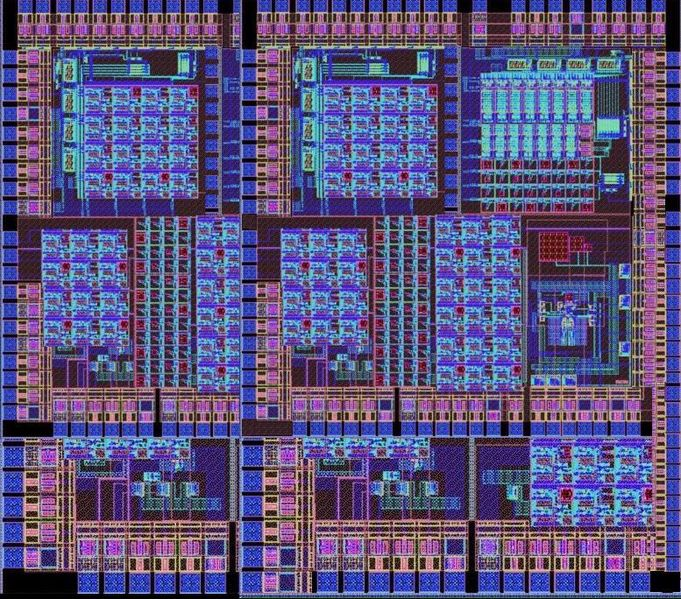
\includegraphics[scale=0.6]{681px-InternalIntegratedCircuit2.jpg}
\caption{Microcircuito produzido pelo processo fotogr�fico de multicamadas. Microprocessador com frequ�ncia de 4.8GHz, utilizado para o processamento de imagens do Gyroscan 6,2 Tesla. \cite{MicroInternal}}
\label{microinternal}
\end{figure}

Como visto acima sabemos que o microprocessador � o cora��o de um sistema microprocessado, na figura \ref{sistemamicro}, defini-se as quatro partes b�sicas de um sistema microprocessado, que incluem um microprocessador, mem�ria e entrada/sa�da que s�o interligados por um sistema de \textit{buses}, que ser� explicado mais a frente. Um \textit{bus} � um conjunto de fios que transmite informa��o entre dois ou mais dispositivos\cite{IntroductionMicro}.

\begin{figure}[h] \centering
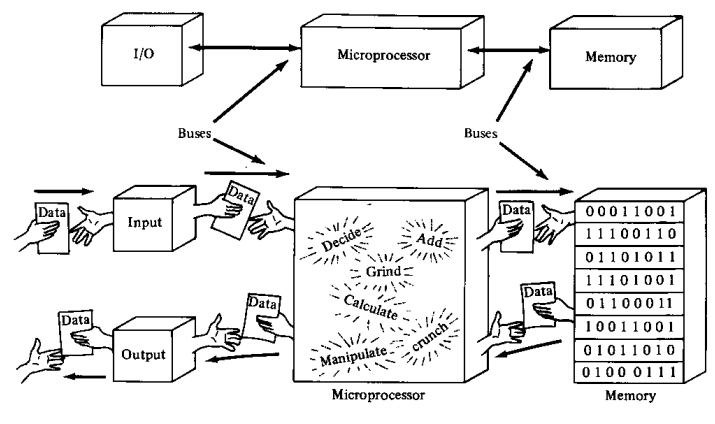
\includegraphics[scale=0.6]{sistemaMicro.png}
\caption{Diagrama de blocos de um sistema microprocessado. \cite{IntroductionMicro}}
\label{sistemamicro}
\end{figure}

\subsection{Funcionamento}
Os microprocessadores funcionam a partir de um rel�gio interno, feito de quartz que quando sujeito a uma corrente el�trica, emite pulsos, chamados de "top". Tais pulsos fazem com que o microprocessador execute uma a��o, ou seja, uma instru��o, seja a mesma executada de forma parcial ou total. Estes pulsos tamb�m definem a pot�ncia do microprocessador, sendo esta pot�ncia definida como o n�mero de instru��es executadas por segundo e tem como unidade utilizada o MIPS (Milh�es de Instru��es Por Segundo) \cite{Microprocessadores}.

Existem dispositivos de entrada e sa�da que permitem a importa��o de dados para armazenamento ou processamento, a exporta��o dos resultados e acessos aos dados armazenados.
Outros sinais importantes para o funcionamento do microprocessador � o sinal de \textit{reset}, que faz com que a CPU volte a um estado inicial que � definido e conhecido, voltando a este estado o microprocessador pode come�ar a executar programas. O sinal de interrup��o faz com que o microprocessador pare sua execu��o e comece a executar uma rotina pr�-definida \cite{Microprocessadores}

\subsection{Programa de Computador}
A figura \ref{programaPC} � uma representa��o visual de um programa de computador, onde ter-se o c�digo n�o � o suficiente. Para realizar a tarefa especificada pelo programa, o computador (microprocessador) necessita ler as instru��es do programa, interpret�-las e execut�-las. \cite{IntroductionMicro}.


\begin{figure}[ht] \centering
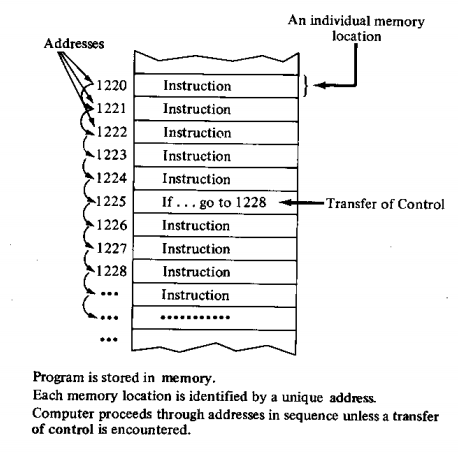
\includegraphics[scale=0.6]{programa.png}
\caption{Organiza��o de um programa de computador \cite{IntroductionMicro}}
\label{programaPC}
\end{figure}

De acordo a \cite{IntroductionMicro} a maneira que um computador executa um programa � c�clica e segue a seguinte ordem:

\begin{enumerate}
\item Leitura (\textit{Fetch}) de uma instru��o
\\Onde o computador l� uma instru��o e a copia da mem�ria para o seu c�rebro (\textit{Microprocessador}).
\item Interpreta��o (\textit{Decode}) da instru��o
\\Cada n�mero que representa uma instru��o dentro do programa, possui um significado para o computador, em termos da a��o que deve ser realizada.
\item Execu��o (\textit{Execute}) da instru��o
\end{enumerate}

Para a realiza��o deste ciclo, o microprocessador conta com uma s�rie de circuitos internos com funcionalidades espec�ficas, que ser�o descritos � seguir.

\subsection{Registradores}
Os registradores s�o utilizados para salvar informa��o bin�ria durante o tempo de execu��o de um programa. Cada registro possui uma fun��o espec�fica associada a ele \cite{ielm}:

O \textbf{acumulador} � um registro prim�rio associado a \textit{ALU} (Unidade L�gica Aritm�tica) e opera��es de entrada/sa�da.
O \textbf{registro de instru��o} guarda o c�digo bin�rio da instru��o que est� sendo executada.
O \textbf{contador de programa} cont�m o endere�o de mem�ria da pr�xima instru��o que deve ser tomada.

Todos estes registradores podem ser visualizados na figura \ref{internalorg}.

\begin{figure}[ht] \centering
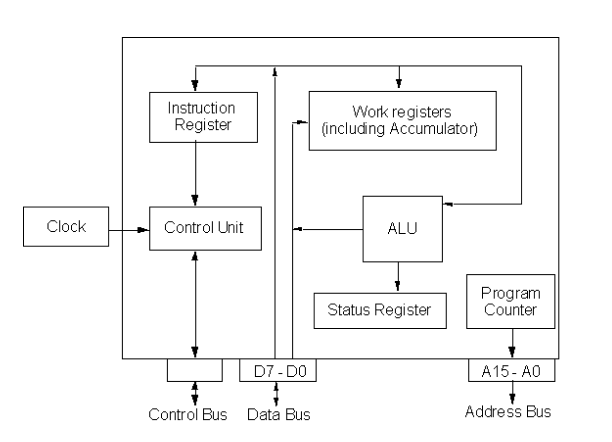
\includegraphics[scale=0.6]{internalOrg.png}
\caption{Organiza��o interna de um microprocessador hipot�tico \cite{ielm}}
\label{internalorg}
\end{figure}

\subsection{Unidade L�gica Aritm�tica}
A Unidade L�gica Aritm�tica, ou \textit{Arithmetic Logic Unit} (ALU) em ingl�s, � o maior componente da unidade central de processamento de um sistema microprocessado. A unidade realiza todos os processos relacionados a opera��es aritm�ticas e l�gicas que necessitam ser feitas nas instru��es. Em alguns microprocessadores a ALU � divida em unidade aritm�tica (UA) e unidade l�gica (UL).
Uma ULA pode ser desenvolvida por engenheiros para calcular qualquer opera��o. Assim que as opera��es come�am a ficar mais complexas, a ULA fica mais cara, ocupa mais espa�o e dissipa mais calor. Por isto,  engenheiros fazem a ULA poderosa o suficiente, para garantir que a Unidade de Processamento seja tamb�m poderosa e r�pida, por�m n�o t�o complexa, que a torne proibitiva em termos de custo entre outras desvantagens \cite{techopediaALU}.

ULAs normalmente realizam as seguintes opera��es:

\begin{itemize}
\item \textbf{Opera��es L�gicas}: Essas incluem AND, OR, NOT, XOR, NOR, NAND, etc.
\item \textbf{Opera��es de Rotacionamento de Bits}: Pertence ao rotacionamento da posi��o dos bits por um certo n�mero de vezes para direita ou esquerda.
\item \textbf{Opera��es Aritm�ticas}: Refere-se, normalmente, a adi��o e subtra��o. Multiplica��o e divis�o as vezes s�o implementadas. Por�m, estas s�o opera��es custosas. A adi��o pode ser utilizada como substituta para a multiplica��o e a subtra��o para a divis�o.
\end{itemize}

\subsection{Unidade de Controle}
A unidade de controle � composta por um controlador de sequ�ncia e um decodificador de instru��o. Durante a execu��o, a unidade de controle, ajusta o conte�do do contador de programa para ser posicionado nas linhas de endere�amento. Essas linhas indicam o endere�o da posi��o de mem�ria, que cont�m o c�digo da pr�xima instru��o a ser executada. Em seguida, a unidade de controle insere no registrador de instru��o o c�digo de instru��o da posi��o de mem�ria. O decodificador de instru��o � habilitado e a unidade de controle ativa as linhas de controle necess�rias, buscando dos resultados desejados \cite{ielm}.

\subsubsection{Sinais de Controle}
Os sinais de controle s�o sinais el�tricos que orquestram as diversas unidades do processador, que participam na execu��o de uma instru��o. Os sinais de controle s�o distribu�dos devido a um elemento chamado sequenciador. O sinal \textit{Read/Write}, em portugu�s Leitura/Escrita, diz para a mem�ria ou outros dispositivos que o processador quer ler ou escrever uma informa��o \cite{Microprocessadores}.

\subsection{Sistema de Barramentos}
No diagrama simplificado da figura \ref{diagramasimp} todos os m�dulos l�gicos se comunicam com a Unidade Central de Processamento. Na pr�tica, muitos modelos de interconex�o podem ser usados, geralmente atrav�s de barramentos. Lembre-se de que um barramento � um meio de transmiss�o de informa��es ou sinais, distinguidos por suas fun��es. No caso dos sistemas baseados em microprocessador, ao menos tr�s barramentos s�o fornecidos \cite{ufpbHardware}:

\begin{itemize}
\item \textbf{Barramento de Dados}: Transmite dados entre as unidades. Portanto, um microprocessador de 8 bits requer um barramento de dados de 8 linhas para transmitir dados de 8 bits em paralelo. Semelhantemente, um microprocessador de 64 bits necessita de um barramento de dados de 64 linhas para transmitir dados de 64 bits em paralelo. Se o barramento de dados para um microprocessador de 64 bits fosse formado por 8 linhas, seriam necess�rias oito transmiss�es sucessivas, tornando mais lento o sistema. O Barramento de Dados � bi-direcional, isto �, pode transmitir em ambas as dire��es.

\item \textbf{Barramento de Endere�o}: � usado para selecionar a origem ou destino de sinais transmitidos em um dos outros barramentos ou numa de suas linhas, conduzindo endere�os. Uma fun��o t�pica do Barramento de Endere�o � selecionar um registrador em um dos dispositivos do sistema, que � usado como a fonte ou o destino do dado. O Barramento de Endere�o do nosso computador padr�o, tem 16 linhas e pode endere�ar $2^{16}$ (64 K) dispositivos (1K = 1024, ou $2^{10}$ , no jarg�o de computa��o).

\item \textbf{Barramento de Controle}: Sincroniza as atividades do sistema, conduzindo o status e a informa��o de controle de/para o Microprocessador. Para um Barramento de Controle ser formado, ao menos 10 (geralmente s�o mais) linhas de controle s�o necess�rias.
\end{itemize}

De acordo a \cite{ufpbHardware}, os barramentos s�o implementados como linhas de comunica��o reais. Eles podem ser posicionados como parte do circuito no pr�prio Chip (Barramentos internos) ou podem servir de comunica��o externa entre os Chips (Barramentos externos). Os barramentos externos podem ser expandidos para facilitar a conex�o de dispositivos especiais. Um projeto eficiente de barramentos � crucial para a velocidade do sistema.


\begin{figure}[ht] \centering
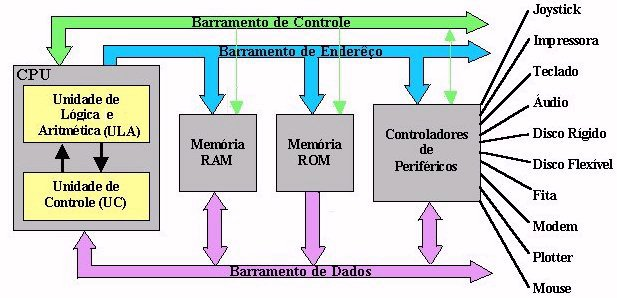
\includegraphics[scale=2.5]{arqBarramento.jpg}
\caption{Diagrama simplificado de um Microcomputador \cite{ufpbHardware}}
\label{diagramasimp}
\end{figure}

\subsection{Dispositivos de Entrada/Sa�da}
Os dispositivos de entrada/sa�da (E/S) ou \textit{input/output (I/O)}, s�o tamb�m denominados perif�ricos, eles permitem a intera��o do processador com o homem, possibilitando a entrada e/ou sa�da de dados.
Por�m, � necess�rio o m�dulo mais a direita da figura \ref{diagramasimp}, que s�o os controladores de perif�ricos. Tais controladores possuem a tarefa de combinar as velocidades entre os dispositivos, pois a maioria dos perif�ricos s�o consideravelmente mais lentos que a unidade de processamento, convertem dados de um formato em outro \cite{ufpbHardware}.
Exemplos de perif�ricos de entrada: teclado, mouse, scanner, etc. Dispositivos de sa�da: monitor, impressora, etc.

\subsection{Arquiteturas}
De acordo com \cite{ComputerOrg}, uma das mais importantes abstra��es � a interface entre o hardware e o software de baixo n�vel. Por causa de sua import�ncia, � dado uma nomenclatura especial: \textbf{arquitetura do conjunto de instru��es} (ISA), ou simplesmente arquitetura de uma m�quina. O conjunto de instru��es, inclui qualquer coisa que programadores necessitam para saber como programar em linguagem de m�quina corretamente, incluem instru��es, dispositivos E/S, entre outros. Tipicamente o sistema operacional ir� encapsular os detalhes da realiza��o da E/S, aloca��o de mem�ria, e outras funcionalidades de baixo n�vel do sistema, portanto, programadores n�o precisam se preocupar com estes detalhes. Dois tipos de conjuntos de instru��es existentes ser�o explicados a diante.

\subsubsection{CISC - Complex Instruction Set Computer}
CISC � uma arquitetura de processador, que teve como princ�pio o uso eficiente de mem�ria e a facilidade de programar. Cada instru��o desse processador tem v�rias opera��es em seu interior ajudando o programador a implementar programas. A maioria dos projetos de microprocessadores comuns - incluindo o Intel (R) 80x86 e s�ries Motorola 68K - tamb�m seguem a filosofia CISC \cite{CISC}.

Os primeiros processadores utilizados para decodificar e executar instru��es, principalmente para trabalhos simples, com poucos registros, funcionaram. Por�m n�o para sistemas complexos. Assim, seus criadores constru�ram uma l�gica simples para controlar os caminhos de dados entre os v�rios elementos do processador, e usou um conjunto simplificado de instru��es de microc�digo para controlar a l�gica do caminho de dados.

A microprograma��o � uma representa��o simb�lica do controle em forma de instru��es, chamadas microinstru��es, que s�o executadas em uma microm�quina simples \cite{ComputerOrg}, podemos ver na figura \ref{microcodigo} o exemplo de um microc�digo.

\begin{figure}[ht] \centering
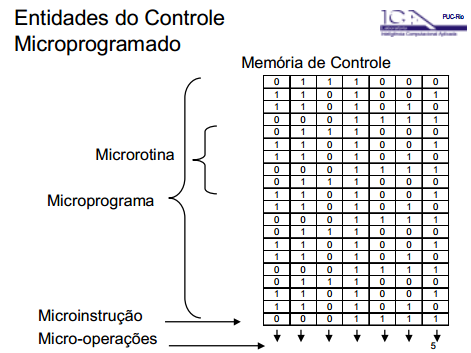
\includegraphics[scale=1]{microcodigo.png}
\caption{Entidades do Controle Microprogramado \cite{pucMicro}}
\label{microcodigo}
\end{figure}


\subsubsection{RISC - Reduced Instruction Set Computer}
Na d�cada de 1980, ocorreu as mudan�as para a nova arquitetura, o modelo RISC (Reduced Instruction Set Computer). As melhorias nas linguagens de programa��o, tecnologia de compiladores e custo de mem�ria significaram que, menos programa��o estava sendo feita no n�vel do assembly, de modo que os conjuntos de instru��es poderiam ser medidos pela forma como os compiladores os usavam, ao contr�rio de como os programadores em assembly os usavam.
Praticamente todos os novos conjuntos de instru��es desde 1982, seguiram essa filosofia RISC de
tamanhos de instru��o fixos, conjuntos de instru��o load/store, modos de endere�amento limitados e
opera��es limitadas. ARM, Hitachi SH, IBM PowerPC, MIPS e Sun SPARC s�o todos exemplos de
arquiteturas RISCs \cite{ComputerOrg}.

\subsubsection{Compara��o entre RISC e CISC}
Como visto anteriormente, a arquitetura CISC apresenta instru��es complexas executadas em v�rios ciclos de clock, enquanto a arquitetura RISC possui somente instru��es que s�o executadas em apenas um ciclo. No quesito de acesso a mem�ria, o conjunto complexo possui v�rios tipos de modos de endere�amento de mem�ria, facilitando o trabalho do programador. Os microprocessadores RISC s�o considerados m�quinas \textit{load/store}, o que � poss�vel pois ele possui uma grande quantidade de registradores dos mais variados tipos. A clara vantagem da arquitetura RISC � em quest�o de velocidade, pois por possuir um conjunto de instru��es, com todas instru��es com formato fixo, ocorre um uso intenso de \textit{pipeline}. No desenvolvimento de um  microprocessador CISC, a complexidade do sistema se encontra no microprograma, como visto um exemplo na figura \ref{microcodigo}, e na arquitetura RISC a complexidade se encontra no compilador. Ambas arquiteturas s�o muito bem aceitas no mercado e cada uma possui suas vantagens e desvantagens para serem aplicados em diversos tipos de projetos.


\subsection{Mem�ria Cache}
De acordo com \cite{memoriacache}, a mem�ria cache consegue realizar a ponte entre a diferen�a de velocidade entre o processador e a mem�ria. A cache � um pequeno espa�o de alta velocidade que se situa entre o processador e a mem�ria na hierarquia de mem�rias.

\begin{figure}[ht] \centering
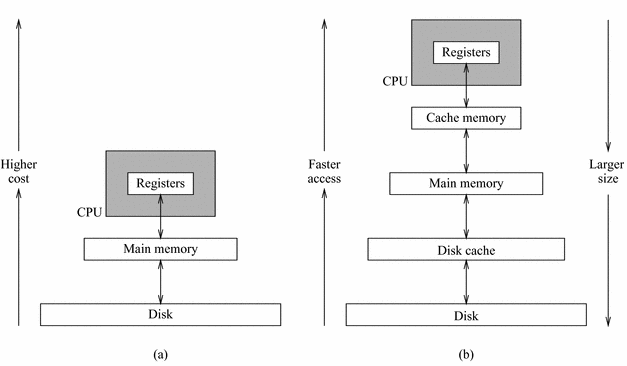
\includegraphics[scale=0.6]{memoriacache.png}
\caption{Hierarquia de Mem�rias \cite{memoriacache}}
\label{memcache}
\end{figure}

Cache, foi o nome escolhido para representar o n�vel na hierarquia de mem�ria entre o processador e a mem�ria do primeiro computador comercial a ter este n�vel extra, como pode ser visto na Figura \ref{memcache} item (b). A raz�o da cache (\textit{SRAM}) ser menor � devido a maiores decodificadores de endere�o, pois s�o mais lentos do que menores decodificadores de endere�o. Quanto maior a mem�ria �, mais complexo � seu decodificador de endere�o, e mais tempo leva para identificar o valor da posi��o de mem�ria do endere�o desejado \cite{memoriacache}.

� poss�vel utilizar este conceito e dar um passo a diante introduzindo uma \textit{SRAM} menor entre o cache o e processador, dentro do pr�prio env�lucro do processador, criando dois n�veis de mem�ria cache L1 e L2, como podemos ver na figura \ref{niveiscache} \cite{memoriacache}.

\begin{figure}[ht] \centering
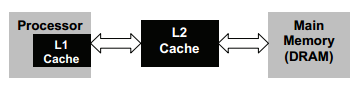
\includegraphics[scale=1]{cacheniveis.png}
\caption{Dois n�veis de mem�ria cache L1 e L2 \cite{memoriacache}}
\label{niveiscache}
\end{figure}

\subsection{Pipeline}
\subsubsection{Defini��o}
De acordo com \cite{ComputerOrg}, \textit{Pipelining} � uma t�cnica de implementa��o no qual multiplas  instru��es s�o sobrepostas durante a execu��o, como visto na figura \ref{pipeline}. Hoje em dia, \textit{pipelining} � a chave para fazer processadores r�pidos \cite{ComputerOrg}.

\begin{figure}[ht] \centering
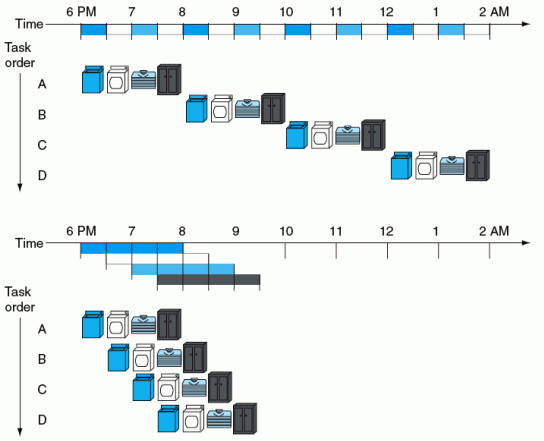
\includegraphics[scale=0.6]{pipeline.png}
\caption{A analogia de uma lavanderia com o pipeline \cite{ComputerOrg}}
\label{pipeline}
\end{figure}

Como podemos ver, a utiliza��o de \textit{pipeline} torna a execu��o muito mais r�pida do que se as tarefas fossem executadas sequencialmente. Como exemplo utilizaremos o microprocessador MIPS, que possui 5 est�gios de execu��o de uma instru��o, sendo elas: Decodifica��o da Instru��o (\textit{Instruction Fetch)}, Leitura dos Registros (\textit{Reg}),Opera��o de ULA (\textit{ALU}) , Acesso ao dado e Escrita no Registro. Na figura \ref{calculoPipeline} podemos ver quantitativamente a diferen�a do processo com utiliza��o de \textit{pipeline}.

\begin{figure}[ht] \centering
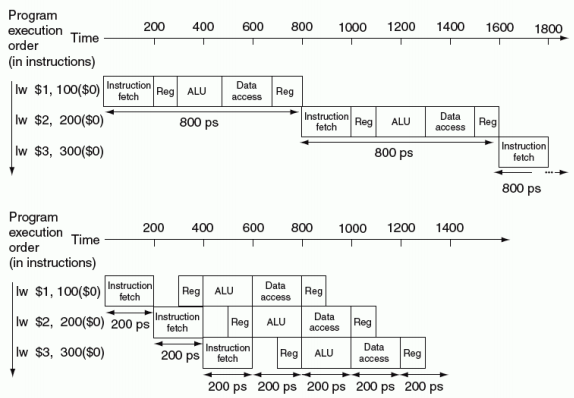
\includegraphics[scale=0.6]{calculoPipeline.png}
\caption{Compara��o quantitativa da utiliza��o de \textit{Pipeline} utilizando a instru��o \textit{Load Word} do microprocessador MIPS. \cite{ComputerOrg}}
\label{calculoPipeline}
\end{figure}

\subsubsection{Desenvolvimento de um conjunto de instru��o para o \textit{Pipeline}}
Primeiramente, todas as instru��es do MIPS possuem o mesmo comprimento, esta restri��o faz com que fique mais f�cil decodificar as instru��es no primeiro e no segundo est�gio  do \textit{pipeline}. Em um conjunto de instru��es, como o do IA-32, onde instru��es variam de 1 at� 17 bytes, o \textit{pipelining} � consideravelmente mais complicado \cite{ComputerOrg}. Atualmente a arquitetura do IA-32 transforma as instru��es em microinstru��es, sendo essas utilizadas para a realiza��o do \textit{pipeline} com uma arquitetura \textit{CISC}.

\subsubsection{Problemas do \textit{Pipeline}}
O \textbf{primeiro} tipo de problema do \textit{pipeline}, � o problema estrutural, que significa que o hardware n�o suporta a combina��o de instru��es ao qual desejamos que sejam executadas em um �nico ciclo de clock. Ao caso de termos somente uma �nica mem�ria, no segundo e quarto passo, s�o necess�rios acessos a mem�ria que n�o podem ser executadas de uma �nica vez \cite{ComputerOrg}.
O \textbf{segundo} tipo de problema , quanto a acesso aos dados, ocorre quando o \textit{pipeline} fica travado no momento em que ocorre uma etapa deve esperar outra etapa completar para continuar, por exemplo no seguinte trecho de c�digo do MIPS, na figura \ref{codigoPipeline}.

\begin{figure}[ht] \centering
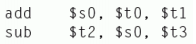
\includegraphics[scale=0.8]{codigo.png}
\caption{Trecho de c�digo que exemplifica um problema do \textit{pipeline} \cite{ComputerOrg}.}
\label{codigoPipeline}
\end{figure}

Quando este tipo de problema ocorre, um fato chamado \textit{bubble} aparece no meio do \textit{pipeline}, como se fosse uma linha vazia entre dois processos do \textit{pipeline}, podendo ser notado na figura \ref{bubble}.

\begin{figure}[ht] \centering
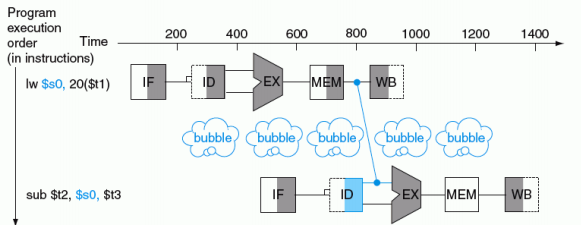
\includegraphics[scale=0.6]{bubble.png}
\caption{Fen�meno do tipo \textit{bubble} no \textit{pipeline} semelhante ao problema da figura \ref{codigoPipeline} \cite{ComputerOrg}.}
\label{bubble}
\end{figure}

Para resolver este tipo de problema, o c�digo pode ser reescrito de uma forma que evite a depend�ncia das informa��es, essa corre��o pode ser realizada tanto pelo compilador como pelo programador.

O terceiro tipo de problema, � chamado de problema de controle, tamb�m chamado de problema de \textit{branch}, surge da necessidade de tomar uma decis�o baseada nos resultados de uma instru��o enquanto outras est�o em execu��o \cite{ComputerOrg}.

As instru��es de \textit{branch} s�o instru��es de desvios condicionais no c�digo, portanto a execu��o da pr�xima instru��o depende se o \textit{branch} causar� desvio ou n�o, caso o desvio ocorra, o fen�meno de \textit{bubble} ocorre novamente, pois o \textit{pipeline} necessita ficar um tempo parado esperando a tomada de decis�o, semelhante a figura \ref{branchproblema}.

\begin{figure}[ht] \centering
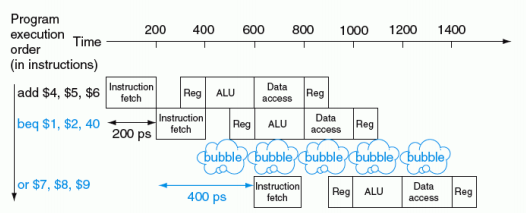
\includegraphics[scale=0.6]{branchproblema.png}
\caption{Fen�meno do tipo \textit{bubble} no \textit{pipeline} quando ocorre o problema de \textit{branch} \cite{ComputerOrg}.}
\label{branchproblema}
\end{figure}

Para solucionar este problema, desenvolveu-se uma estrutura dentro do pr�prio microprocessador, chamada \textit{branch predictor}. O \textit{branch predictor} � um circuito digital que tenta adivinhar qual vai ser o caminho que o branch ir� seguir, para continuar preenchendo o \textit{pipeline}. Hoje em dia, tal estrutura desempenha um papel fundamental para o desenvolvimento de processadores de alta performance.


\subsection{Processadores Multi-Core e Hyper-Threading}
De acordo com \cite{intelMulticore}, basicamente, multi-core � um design ao qual um �nico processador f�sico, cont�m o n�cleo l�gico de mais de um processador, como pode ser visto na figura \ref{multicore}. O objetivo deste design � habilitar o sistema a executar mais tarefas simultaneamente e desse modo alcan�ar um maior desempenho do sistema.

\begin{figure}[ht] \centering
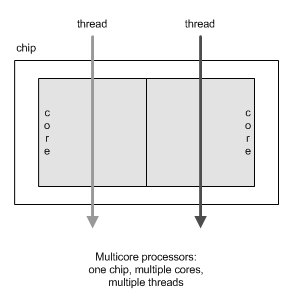
\includegraphics[scale=1]{multicore.png}
\caption{Processador com dois n�cleos dentro de um �nico processador \cite{intelMulticore}.}
\label{multicore}
\end{figure}


Programas s�o executados, � partir de threads, essas threads s�o sequ�ncias de instru��es relacionadas. Nos prim�rdios do PC, a maioria dos programas consistia de uma �nica thread, o sistema operacional naquela �poca  era capaz de executar somente um programa por vez, tendo como resultado uma sensa��o dolorosa que seu PC congelava enquanto imprimia um documento ou uma folha de trabalho, o sistema era incapaz de realizar duas tarefas simultaneamente. Inova��es no sistema operacional introduziram os sistemas multitarefa, no qual um programa pode ser brevemente suspendido enquanto executa outro, de uma maneira que o usu�rio n�o perceba. Realizando esta troca rapidamente, o sistema tem a apar�ncia de estar executando os programas simultaneamente, contudo o processador estava de fato, executando uma �nica thread.

No in�cio dos anos 2000, o design de processadores ganhou recursos adicionais, como uma l�gica dedicada para opera��es com ponto flutuante, para suportar a execu��o de m�ltiplas instru��es em paralelo. A Intel\textregistered, definiu que o melhor uso desses recursos empregando-as para executar duas threads simultaneamente no mesmo n�cleo de processamento, figura \ref{hyperthreading}. A Intel\textregistered  nomeou este procedimento simult�neo como \textit{Hyper-Threading Technology}\textregistered e lan�ou-a nos processadores \textbf{Intel Xeon \textregistered} em 2003. De acordo com medidores da Intel\textregistered, aplica��es que eram escritas utilizando m�ltiplas threads realizaram suas tarefas 30\% mais r�pido do que se for executado utilizando a tecnologia \textbf{HT}. Para induzir o sistema operacional a reconhecer um processador como duas possibilidades de execu��o de \textit{pipeline}, \textit{chips} foram feitos para aparentar ser dois processadores l�gicos.

\begin{figure}[ht] \centering
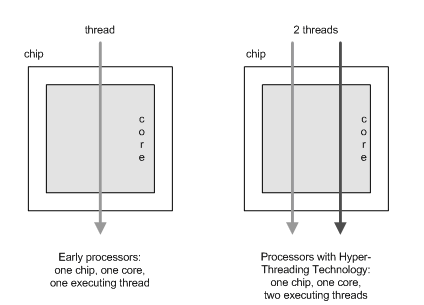
\includegraphics[scale=1]{Hyperthreading.png}
\caption{Exemplo de um processador com a tecnologia \textit{Hyper-Threading} \cite{intelMulticore}.}
\label{hyperthreading}
\end{figure}


\section{Microprocessador 8086/8088}
\subsection{Hist�ria}

\quad Em 1968 a empresa Intel foi fundada por Robert N. Noyce, Gordon E. Moore e Andrew Grove. Robert N. Noyce foi o inventor do circuito integrado.

Em 15 de novembro de 1971 nascia o processador 4004 de apenas 4 bits e grande capacidade para realizar opera��es aritm�ticas. Esse microprocessador possu�a 2.300 transistores para processar 0,06 milh�es de instru��es (60.000) por segundo e n�o tinha o tamanho de um selo de carta.  Para se ter uma id�ia, o ENIAC, primeiro computador de que se tem not�cia , constru�do em 1946 para fins b�licos, ocupava sozinho 1.000 metros quadrados e fazia o mesmo que o 4004.

O 4004 foi usado apenas para c�lculos poucos complexos (4 opera��es), ele era um pouco mais lento que o  Eniac II mais tinha a vantagem de possuir a metade do tamanho, esquentar menos e consumir menos energia.

	Surgiu em 1972 o 8008, primeiro processador de 8 bits, com capacidade de mem�ria de 16 Kbytes (16.384 bytes), enquanto o 4004 possu�a apenas 640 bytes.
	
	Em 1974 � lan�ado o 8080, com desempenho seis vezes maior que o anterior com um clock de 2 MHz, rodava um programa da Microsoft chamado Basic, possu�a apenas led's. Al�m de 16KB de mem�ria ROM onde ficava o sistema, possu�a 4KB de mem�ria RAM, seus controles eram atrav�s de bot�es, possu�a drive de disquete 8"    com capacidade de 250 KB.
	
	O 8086 foi o primeiro processador feito pela Intel para ser usado com os PC's. Ele contava com um barramento de dados interno e externo de 16 bits. E foi este  o motivo de n�o ter sido o processador mais utilizado. Inicialmente ele foi distribu�do em vers�es de 4,77 MHz. Posteriormente vieram vers�es turbinadas de 8 e 10 MHz. 
	
	A hist�ria do 8086 � bem simples. Quando ele foi lan�ado, a maioria dos dispositivos e circuitos dispon�veis eram de 8 bits. Era muito caro adaptar todo o resto do computador por causa do processador. E foi isso que acabou com o  8086. Para adaptar-se a este mercado a Intel lan�ou o 8088, com barramento externo mais lento, de 8 bits. Deixando a diferen�a de barramento externo, ambos eram id�nticos. 
	
	Quando este chip, o 8086, veio a ser utilizado j� era tarde demais. Ele chegou at� a fazer parte de uns poucos clones do IBM PC e posteriormente em dois modelos do IBM PS/2 e de um computador Compaq. Mas sua destrui��o veio com um processador mais poderoso, o 80286. 
	
	Outro poss�vel fator para a pouca aceita��o deste processador pode ter sido a falta de unidades devido � demanda. Nunca havia chips suficientes para produzir computadores em grande escala.

\subsection{Vis�o preliminar}
\quad Tanto o 8086 como o 8088 utilizam o conceito de fila de instru��es para melhorar a velocidade do computador. Uma �rea no interior da pastilha denominada fila de instru��es ret�m diversos bytes de uma instru��o. Quando o computador estiver pronto para a pr�xima instru��o, ele n�o precisa pegar muitos bytes na mem�ria, uma vez que toda instru��o poder� j� se encontrar na fila. O conceito de fila aumenta o numero de opera��es realizadas por segundo uma vez que o processador vai estar utilizando o bus de dados e endere�os por menor per�odo de tempo, disponibilizando este para outros dispositivos. A fila do 8086 tem 6 bytes de largura e a do 8088 tem 4 bytes.

	O 8086 pode acessar 1 megabyte de mem�ria de leitura/escrita ($2^{20}$ bytes). Entretanto ele utiliza um esquema de endere�amento de mem�ria denominado segmenta��o, em que determinados registradores de segmento fornecem um endere�o b�sico que � automaticamente acrescentado a cada endere�o de usu�rio de 16 bits na m�quina.

\begin{figure}[h!] \centering
		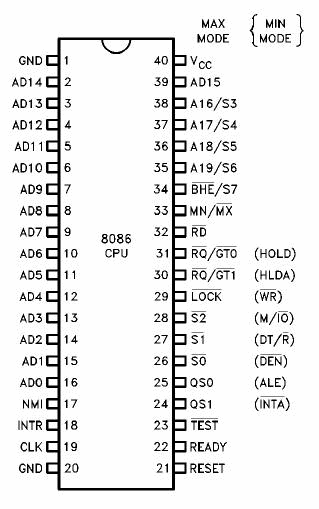
\includegraphics[scale=0.5]{pinagem.png}
		\caption{Pinagem do IA-PX 86 \cite{micro8086}}
		\label{diagrama}
	\end{figure}

A parte do endere�o e todas as vias de dados s�o multiplexados em 16 pinos (os 16 pinos do barramento de dados � o que o classifica como um microprocessador de 16 bits). Os 4 bits restantes s�o implementados por quatro pinos adicionais de endere�o, que tamb�m s�o utilizados para status (como mostra a figura 16). � requerido um clock externo � pastilha e � utilizado um controlador de via externo � pastilha para demultiplexar a via de dados e de endere�o.

\begin{figure}[h!] \centering
		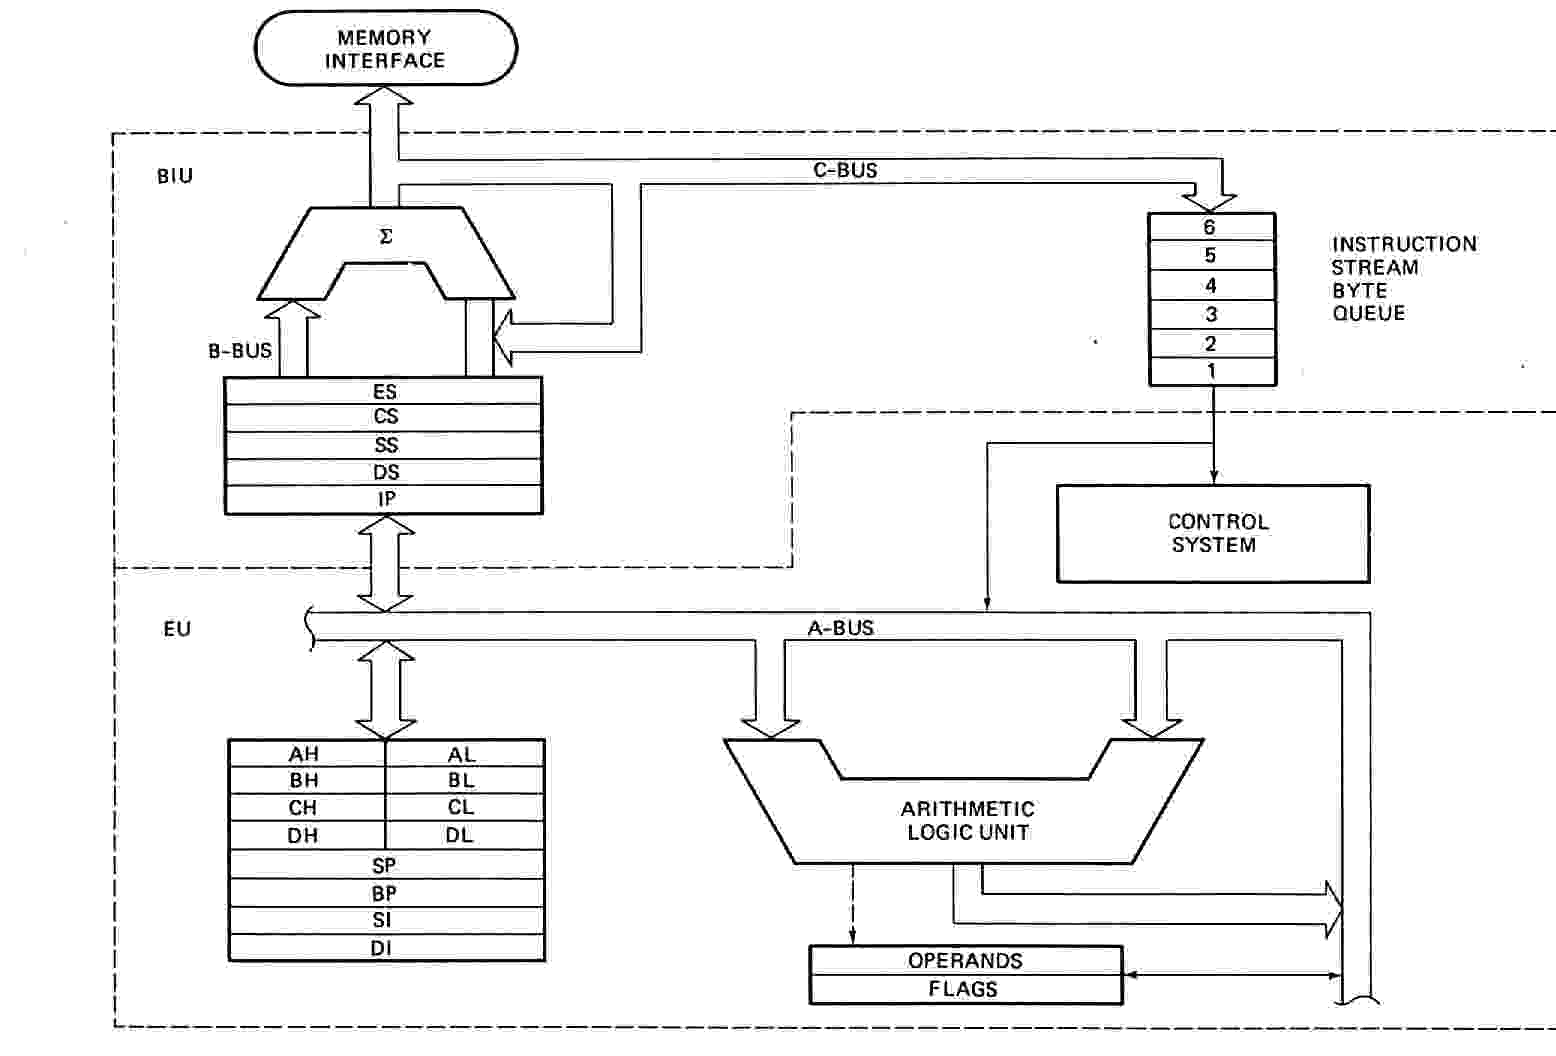
\includegraphics[scale=0.5]{intern_diagram.png}
		\caption{Arquitetura do 8086/8088 \cite{micro8086}}
		\label{diagrama}
	\end{figure}
	
	O 8086 tem uma estrutura de interrup��o poderosa. Quase todos os microprocessadores de 8 bits requerem pastilhas externas adicionais para permitir opera��es de interrup��o adequadas. No 8086, cerca de 1000 bytes s�o colocados de lado para conter at� 265 apontadores de vetores (lembrando que cada apontador � um endere�o contendo seletor:offset, ou seja, 4 bytes). O 8086 executa opera��es de E/S (ou I/O) em um espa�o separado da mem�ria denominado espa�o de E/S. Tem um total de 64 KBytes. Para ser utilizado pelos co-processadores � fornecido um pino de entrada TEST especial (pino 23, figura 16) para permitir ao 8086 saber quando � que o co-processador completou a tarefa. Quando uma instru��o WAIT � acionada, o 8086 p�ra e aguarda do co-processador externo, ou qualquer outro hardware, um sinal para que continue pela altera��o do pino TEST.
	
\subsection{Mem�ria}
\quad A largura de mem�ria "vista" por um microprocessador � determinada pela quantidade de bits que o microprocessador pode acessar por vez. Esta quantidade � determinada pela largura do seu barramento de dados externo. O microprocessador 8086 possui um barramento de dados de 16  bits o que permite acessar dois bytes da mem�ria consecutivamente (cada refer�ncia � mem�ria acessa 2 bytes), enquanto, o 8088 possui um barramento de dados de 8 bits, ou seja, uma refer�ncia � mem�ria acessa 1 byte.

	Os microprocessadores 8086/8088 podem acessar (ler ou escrever) bytes ou palavras (2 bytes) que se localizam tanto em endere�os pares como em endere�os �mpares da mem�ria. No entanto, dependendo do microprocessador e do tamanho do dado a ser acessado, pode ser necess�rio que o microprocessador efetue uma ou duas refer�ncias para a mem�ria. A tabela 1 resume o n�mero de refer�ncias necess�rias para os microprocessadores 8086/8088 acessarem dados de 8 e 16 bits em endere�os pares e �mpares da mem�ria.
\begin{center}
\begin{table}[htbp]
  \centering
  \caption{N�mero de Refer�ncias 8086/8088}
    \begin{tabular}{|c|c|cccc|}
    \hline
    \multirow{2}[4]{*}{Tamanho do Dado} & \multirow{2}[4]{*}{Endere�o} & \multicolumn{4}{c|}{N�mero de Refer�ncias} \\
          &       & \multicolumn{2}{c}{8086} & \multicolumn{2}{c|}{8088} \\
          \hline
    \multirow{2}[4]{*}{Byte} & Par   & \multicolumn{2}{c}{1} & \multicolumn{2}{c|}{1} \\
          & Impar & \multicolumn{2}{c}{1} & \multicolumn{2}{c|}{1} \\
          \hline
    \multirow{2}[4]{*}{Palavra} & Par   & \multicolumn{2}{c}{1} & \multicolumn{2}{c|}{2} \\
          & Impar & \multicolumn{2}{c}{2} & \multicolumn{2}{c|}{2} \\
    \hline
    \end{tabular}%
  \label{tab:addlabel}%
\end{table}%

\end{center}
O espa�o de endere�amento da mem�ria do microprocessador 8088 � organizado como um vetor linear de 1 MByte, sendo que cada localiza��o deste espa�o � referenciada por meio de um endere�o �nico de 20 bits chamado endere�o f�sico.

	No microprocessador 8086 o espa�o de endere�amento da mem�ria � organizado em dois bancos de 512 KBytes cada, chamados bancos par e �mpar, respectivamente. O banco par � conectado ao 8086 por meio de 8 bits menos significativos do barramento de dados, j� o banco �mpar � conectado por meio dos 8 bits mais significativos do barramento de dados. 

\subsection{Arquitetura do microprocessador}

\quad A unidade de execu��o (EU) executa as opera��es aritm�ticas e l�gicas, al�m de controlar a maioria dos registros internos e manipular os dados. Em contraste, a unidade de interface de barramento (BIU representado por um s�mbolo de somat�ria na figura 17) executa as opera��es de barramento, incluindo a transfer�ncia de dados, e controla os registros restantes do microprocessador.

	As duas unidades de processamento s�o capazes de executar suas opera��es de forma independente, isto �, cada unidade pode fazer suas tarefas sem a assist�ncia da outra unidade.
	
	Embora a unidade de execu��o EU esteja isolada do barramento do sistema, pela unidade de interface de barramento (BIU), ela ainda pode acessar o barramento para certas opera��es. A EU ganha o acesso do barramento requisitando que a BIU temporariamente suspenda suas atividade. A EU ent�o assume o controle da BIU de modo a poder usar o barramento para enviar ou receber informa��es.
	
	Da figura 17 nota-se que a EU consiste de duas se��es principais que s�o os registros de prop�sitos gerais e a unidade aritm�tica e l�gica - ALU. Os registros de prop�sito geral do 8086/8088 presentes na EU s�o �reas de armazenamento com capacidade de manter dados bin�rios que foram ou ser�o usados pelo microprocessador. A grande vantagem destes registros se deve ao fato de se poder acess�-los com maior facilidade e de forma muito mais r�pida do que uma determinada localiza��o da mem�ria.
	
	Todos os registros de prop�sito geral possuem capacidade aritm�tica e l�gica. Dados podem ser armazenados atrav�s da BIU ou transferidos para mem�ria. Os registros de prop�sito geral s�o todos de 16 bits, entretanto os bytes menos e mais significativos podem ser usados separadamente como registros de 1 byte, dessa forma tem-se os seguintes registros: AH, AL, BH, BL, CH, CL, DH e DL.
	
	A maioria das opera��es que se pode executar em um dos registros de prop�sito geral podem tamb�m ser executadas nos demais registros. Contudo, os registros de prop�sito geral tem uso espec�fico para algumas poucas instru��es. Devido a este fato, os registros de prop�sito geral recebem nomes descritivos que s�o: Acumulador (AX), Base (BX), Contador (CX), Dado (DX), �ndice fonte (SI), �ndice destino (DI), ponteiro base (BP) e ponteiro da pilha (SP).
	
	A unidade aritm�tica e l�gica, ALU, recebe instru��es e ent�o executa sobre os dados especificados pela instru��o uma opera��o aritm�tica, como soma ou subtra��o ou l�gica como OR ou AND.
	
	A se��o de l�gica de controle de barramento � respons�vel por todas as opera��es de barramento do microprocessador como, por exemplo, a busca de dados para a unidade aritm�tica e l�gica (ALU). Quando necess�rio a se��o de l�gica de controle de barramento acessa localiza��es particulares na mem�ria, de modo que a EU possa enviar ou receber informa��es para ou destas localiza��es.
	
	A se��o de l�gica de controle de barramento tamb�m controla o sentido do fluxo de informa��o no barramento. Quando uma informa��o tiver que ser enviada � mem�ria, esta se��o assegura que os sinais de controle sejam os apropriados para a transmiss�o. O mesmo ocorre quando for necess�rio receber uma informa��o. A fila de instru��es age como um "encanamento" onde os bytes das instru��es trazidos da mem�ria s�o armazenados antes do seu uso pela EU. No 8086 esta fila � composta de 6 localiza��es de 8 bits cada, enquanto no 8088 a fila de instru��es � composta de 4 localiza��es de 8 bits. Pode-se dizer que estas localiza��es servem como �reas para o armazenamento tempor�rio (buffer) das instru��es trazidas da mem�ria.
	
	No microprocessador 8086/8088 � a se��o l�gica de controle de barramento BIU, que busca os bytes das instru��es do programa na mem�ria e os coloca na fila de instru��es. Esta fila mant�m estes bytes at� que a EU esteja pronta para aceit�-las.
	
	Devido as caracter�sticas do microprocessador 8086, a BIU sempre busca as instru��es acessando palavras (16 bits) que se encontram armazenadas em endere�os pares. A �nica exce��o ocorre quando existe um desvio (JUMP) para uma instru��o que se encontra armazenada na mem�ria em um endere�o impar. Quando isso ocorre o 8086 traz para a fila de instru��es um �nico byte da instru��o e a seguir continua acessando palavras que se encontram armazenadas em endere�os pares. Este fato n�o ocorre em um 8088 visto que seu barramento de dados � de 8 bits. � importante salientar que as instru��es de um microprocessador 8086 podem ter de um a seis bytes de comprimento.
	
	Independente do microprocessador, caso ocorra um desvio na seq��ncia de execu��o das instru��es, a fila de instru��es � automaticamente esvaziada e a BIU passa a buscar as instru��es a partir da nova localiza��o de mem�ria para a qual se deu o desvio. 

\subsection{Endere�amento da mem�ria}

\quad Ao contr�rio dos microprocessadores que utilizam um modelo de mem�ria linear, ou seja, que enxergam o seu espa�o de endere�amento de mem�ria de forma sequencial, o 8086/8088 utiliza um modelo de mem�ria denominado segmentada. Neste modelo o microprocessador enxerga o espa�o de endere�amento de mem�ria dividido em v�rios segmentos.

	Um segmento nada mais � do que uma regi�o continua do espa�o de endere�amento de mem�ria que � tratada pelo microprocessador como uma unidade l�gica. Por serem unidades l�gicas e n�o f�sicas, os segmentos podem localizar-se em qualquer parte do espa�o de endere�amento linear. Conseq�entemente, dois ou mais segmentos distintos podem ser: adjacentes, parcialmente sobrepostos, totalmente sobrepostos ou desconexos.
	
	No modelo de mem�ria segmentada do 8086/8088, o microprocessador somente pode acessar as localiza��es de seu espa�o de endere�amento por meio de um determinado segmento. Assim para este microprocessador, um segmento funciona como uma "janela m�vel" sobre o seu espa�o de endere�amento linear, atrav�s do qual ele acessa as localiza��es do seu espa�o de endere�amento.
	
	Para o microprocessador 8086/8088, os segmentos podem se localizar em qualquer parto do seu espa�o de endere�amento de mem�ria. Entretanto, devido a arquitetura deste microprocessador, um seguimento somente pode come�ar em uma localiza��o do espa�o de endere�amento de mem�ria, cujo endere�o f�sico seja m�ltiplo de 16 (10H).
	
	O endere�o f�sico do in�cio de um segmento do 8086/8088 � designado por endere�o base, os 16 bits mais significativos do endere�o base correspondem a um endere�o chamado endere�o de segmento ou seletor. Conseq�entemente, cada segmento do 8086/8088 � identificado por um endere�o de segmento ou seletor de 16 bits.
	
	Dentro de cada segmento o endere�amento se da de forma linear, por�m relativo ao endere�o de in�cio do segmento. Cada localiza��o do espa�o de endere�amento de mem�ria dentro do segmento � identificado por meio de um endere�o de 16 bits chamado endere�o efetivo (Effective Address - EA) ou endere�o de offset (offset).
	
	Devido a segmenta��o do espa�o de endere�amento de mem�ria e ao endere�amento relativo dentro do segmento, cada localiza��o do espa�o de endere�amento de mem�ria do microprocessador � identificado por meio de um endere�o de 32bits chamado de endere�o l�gico (seletor : offset).
	
	A forma como o microprocessador converte um endere�o l�gico de 32 bits em um endere�o f�sico de 20 bits, faz com que v�rios endere�os l�gicos identifiquem uma mesma localiza��o do espa�o de endere�amento de mem�ria. A convers�o de endere�o l�gico em endere�o f�sico se da multiplicando o seletor por 10h e em seguida somando o offset. O endere�o f�sico pode ser representado na forma normalizada para obter-se o endere�o l�gico, os 4 bits menos significativos do endere�o f�sico correspondem ao endere�o de offset e os 16 bits mais significativos do endere�o f�sico correspondem ao endere�o de segmento.


\subsection{Conjunto de registros}

\quad Embora os registros SI, DI, BP e SP possuam capacidade aritm�tica e l�gica de 16bits, como os demais registros de prop�sito geral de 16 bits, estes registros geralmente s�o usados para manter o endere�o efetivo (offset) de localiza��es de mem�ria ou para apontar estruturas de dados na mem�ria.

	Particularmente, o registro SP � utilizado para manter o endere�o efetivo do topo de uma estrutura de dados na mem�ria que funciona como uma pilha (stack), onde o �ltimo dado a ser armazenado nesta estrutura dever� ser o primeiro a ser retirado (LIFO - Last Input/first output). Uma vez que esta estrutura � de vital import�ncia para o funcionamento do microprocessador, a utiliza��o do registro SP em opera��es aritm�ticas ou l�gicas n�o � aconselhada.
	
	Como o microprocessador 8086/8088 utiliza um modelo de mem�ria segmentada, o acesso �s localiza��es do seu espa�o de endere�amento de mem�ria � feito atrav�s de segmentos mediante endere�os l�gicos de 32bits. Por isso, para poder acessar as localiza��es dentro de um determinado segmento � necess�rio que o 8086/8088 conhe�a o endere�o deste segmento, ou seja, o seu seletor. Para isso, o microprocessador 8086/8088 disp�e de um conjunto de registros especiais chamados registro de segmentos, cuja finalidade, como o pr�prio nome indica, � manter endere�os de segmentos.
	
	Para acessar uma localiza��o do espa�o de endere�amento de mem�ria que n�o � abrangida por um dos segmentos apontados pelos registros de segmentos, � necess�rio alterar o conte�do de um dos registros de segmento, de modo que este registro aponte para um segmento que venha a abranger a localiza��o que se deseja acessar.
	
	Um programa, geralmente, � composto por tr�s partes ou segmentos que s�o: segmento de c�digos, segmento de dados e segmento de pilha. As partes ou segmentos de um programa podem residir em qualquer ordem e em qualquer lugar do espa�o de endere�amento de mem�ria que tenha mem�ria f�sica.
\\
\\
% Table generated by Excel2LaTeX from sheet 'Plan1'
\begin{center}
\begin{tabular}{|c|r|r|}
\hline
Parte do programa & Registro de segmento \\
\hline
C�digo do programa &         CS \\
\hline
Dados do programa &         DS \\
\hline
Pilha do programa &         SS \\
\hline
�rea extra da mem�ria &         ES \\
\hline
\end{tabular}  
\end{center}
O ponteiro de instru��es (IP) � um registro de 16 bits, que sempre mant�m o endere�o efetivo da localiza��o de mem�ria onde est� armazenado o c�digo de m�quina da pr�xima instru��o a ser executada. Este registro � automaticamente incrementado pelo microprocessador de acordo com o tamanho desta instru��o.

	A representa��o de um endere�o l�gico se d� na forma seletor:offset. Quando os conte�dos de dois registros s�o usados para especificar um endere�o l�gico, o endere�o l�gico geralmente � escrito na forma RS:RO onde RS corresponde ao nome do registro que mant�m a parte do endere�o l�gico que se refere ao endere�o de segmento e RO corresponde ao nome do registro que mant�m a parte do endere�o l�gico que se refere ao endere�o efetivo (offset). Os registros que podem ser utilizados para apontar localiza��o dentro do segmento de dados s�o os registros BX, SI e DI.
	
	No segmento de stack o ponteiro de stack (SP) mant�m o endere�o efetivo da localiza��o de mem�ria que corresponde ao topo da pilha. O endere�o de segmento � mantido no registro de segmento SS.
	
	O poder real de um microprocessador est� na sua capacidade de tomar decis�es. O 8086/8088 baseia as suas decis�es no conte�do de um registro de 16 bits chamado registro de flags. Este registro � automaticamente atualizado para manter informa��es a respeito da ultima opera��o aritm�tica ou l�gica que o microprocessador executou. Apenas 9 flags do registro de flags s�o utilizados, s�o eles: OF - overflow, DF - dire��o, IF - interrup��o, TF - armadilha, SF- sinal, ZF - zero, AF - carry auxiliar, PF- paridade e CF - carry.

\subsection{Instru��es}

\quad Cada instru��o (cart�o de referencia do microprocessador 8086/8088 em anexo) possui uma representa��o bin�ria �nica que � conhecida por c�digo de m�quina. Este modelo bin�rio ou c�digo de m�quina da instru��o, quando for aplicado aos circuitos internos do microprocessador faz com que ele execute uma opera��o particular. Uma instru��o de um modo geral pode ser dividida em duas partes: c�digo de opera��o (opcode) e operandos. 

	O c�digo de opera��o (opcode) � a parte da instru��o que identifica a opera��o b�sica a ser executada pelo microprocessador. Enquanto, os operandos identificam os dados que devem ser utilizados.
	
	Dependendo da instru��o ela pode ter 2 operandos, 1 operando ou nenhum operando. Na representa��o das instru��es com dois operandos, o operando destino � sempre especificado em primeiro, e este � separado do operando fonte por uma v�rgula.
	Quando um operando se refere a um registro de 8 ou 16 bits ele � chamado de operando registro, e quando ele refere a uma localiza��o de mem�ria ele � chamado operando mem�ria. Por outro lado, um operando imediato se refere a um dado de 8 ou 16 bits que � especificado na pr�pria instru��o.
	
	Um operando pode se encontrar em um registro (operando registro), numa localiza��o de mem�ria (operando mem�ria), num dispositivo perif�rico de entrada/sa�da, ou at� mesmo estar codificado no pr�prio c�digo de m�quina da instru��o (operando imediato). A maneira na qual a localiza��o de um operando � especificada chama-se modo de endere�amento.
	O 8086/8088 utiliza duas categorias de endere�amento geral que s�o, o modo de endere�amento registro ou modo registro e o modo de endere�amento mem�ria ou modo mem�ria. Pode-se dizer que uma instru��o do 8086/8088 utiliza o modo de endere�amento registro quando nenhum dos operandos da instru��o se refere a mem�ria. Por outro lado, uma instru��o utiliza o modo de endere�amento mem�ria quando um dos operandos se refere a um operando mem�ria.
	
	Quando se trata de um operando mem�ria at� 3 valores de 16 bits podem ser somados para especificar seu endere�o efetivo. Nesta soma qualquer carry que venha a ocorrer � ignorado pelo microprocessador, por um endere�o efetivo (offset) no 8086/8088 � representado por um n�mero de 16 bits.
	
	Sobre as 2 categorias gerais de endere�amento existem 7 modos espec�ficos de endere�amento.

\subsubsection{Endere�amento por registro}

\quad Uma instru��o utiliza o modo de endere�amento por registro quando os operandos fonte e destino forem registros.

Exemplo: MOV AX, BX.

\subsubsection{Endere�amento imediato}

\quad Uma instru��o utiliza o modo de endere�amento imediato quando o operando fonte desta instru��o for imediato. 
	
	Exemplos: MOV CX, 1234h (modo registro); MOV [2011H], 1234H (modo mem�ria).
	
\subsubsection{Endere�amento Direto}

\quad Uma instru��o utiliza o modo de endere�amento direto quando o operando destino ou operando fonte da instru��o se refere a uma localiza��o de mem�ria, cujo endere�o efetivo � especificado na pr�pria instru��o. 
	
Exemplos: MOV CX, [1234H]; MOV [1234H], DX

\subsubsection{Endere�amento indireto por registro}

\quad Uma instru��o utiliza o modo de endere�amento indireto por registro quando o operando destino ou o operando fonte da instru��o se refere a um operando mem�ria, cujo endere�o efetivo se encontra armazenado num registro.
	
Exemplo: MOV CX, [BX];

\subsubsection{Endere�amento por base}

\quad Uma instru��o utiliza o modo de endere�amento por base quando o operando destino ou operando fonte da instru��o se refere a um operando mem�ria, cujo endere�o efetivo (EA) � especificado pela soma do conte�do do registro BX ou BP com um n�mero de 8 ou 16 bits chamado deslocamento. No caso do deslocamento de 8 bits o microprocessador estende o sinal at� se obter um numero bin�rio sinalizado de 16 bits, quando ocorrer um deslocamento de 16 bits o microprocessador interpreta como um numero absoluto de 16 bits.

		Quando o conte�do do registro BP � utilizado no c�lculo, o 8086/8088 automaticamente associa o endere�o efetivo do operando mem�ria com o conte�do do registro de segmento de stack (registro SS), de modo a formar o endere�o l�gico do operando mem�ria. Neste caso, portando, o 8086/8088 acesa o operando mem�ria no segmento da pilha. 

Exemplo: MOV AX, [BX + 1000H]

\subsubsection{Endere�amento Indexado}

\quad Uma instru��o utiliza o modo de endere�amento indexado quando o operando destino ou o operando fonte da instru��o se refere a um operando mem�ria, cujo endere�o efetivo � especificado pela soma do conte�do do registro SI ou DI, com um n�mero bin�rio de 8 ou 16 bits chamado deslocamento. No caso do deslocamento de 8 bits o microprocessador estende o sinal at� se obter um n�mero bin�rio sinalizado de 16 bits, quando ocorrer um deslocamento de 16 bits o microprocessador interpreta como um n�mero absoluto de 16 bits.

Exemplo: MOV AX, [SI + 2000H]

\subsubsection{Endere�amento por base indexado}

\quad Uma instru��o utiliza o modo de endere�amento por base indexado quando o operando destino ou o operando fonte da instru��o se refere a um operando mem�ria, cujo endere�o efetivo � especificado pela soma do conte�do do registro BX ou BP, com o conte�do do registro SI ou DI e opcionalmente um n�mero bin�rio de 8 ou 16 bits chamado deslocamento.
		
Exemplo: MOV AX, [BX + SI + 2000H]

\section{VHDL}
A linguagem VHDL foi desenvolvida pela necessidade de um padr�o para o interc�mbio de informa��es entre 			fornecedores de equipamentos para o Departamento de Defesa dos Estados Unidos. Esta linguagem � usada para descrever o comportamento de circuitos ou sistemas eletr�nicos a partir de um sistema f�sico. � importante lembrar que esta � uma linguagem concorrente, ou seja, os comandos envolvidos em um mesmo evento acontecem simultaneamente, diferentemente de linguagens de programa��o de software.  Al�m disso, � uma linguagem port�vel, ou seja,  independe da tecnologia ou do fornecedor. A Figura 18 mostra as etapas de um projeto utilizando VHDL.

	\begin{figure}[h] \centering
		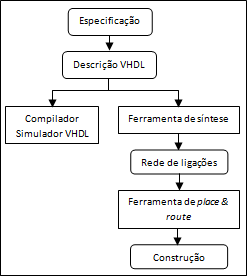
\includegraphics[scale=0.7]{etapa_projeto_vhdl.png}
		\caption{Etapas de Projeto Usando VHDL}
		\label{etapaProjeto}
	\end{figure}											
											
Na l�gica program�vel, h� dois dispositivos principais: CPLD (\emph{Complex Programmable Logic Devices}) e FPGA (\emph{Field Programmable Gate Arrays}) no campo de ASIC (\emph{Application Specific Integrated Circuits}). A partir do c�digo VHDL, pode-se fabricar um chip de alta complexidade ou execut�-lo em um dispositivo program�vel.

O c�digo VHDL � composto de tr�s partes principais: Biblioteca, Entidade e Arquitetura.
\begin{enumerate}
    \item Biblioteca (\emph{Library}) : � composta de todas as bibliotecas usadas no projeto.
    \item Entidade (\emph{Entity}): Determina as entradas e sa�das do circuito.
    \item Arquitetura (\emph{Architecture}): Cont�m o c�digo VHDL que descreve a forma como o circuito deve se comportar (\emph{function}).
\end{enumerate}

\subsection{Biblioteca}
Uma biblioteca t�m v�rias implementa��es de c�digo que s�o �teis a outros projetos. A Figura \ref{library} ilustra a estrutura t�pica de uma biblioteca. O c�digo, normalmente, � escrito na forma de fun��es (\emph{Functions}), procedimentos (\emph{Procedures}) ou componentes (\emph{Components}), que ficam dentro de pacotes (\emph{Packages}) e depois � compilado na biblioteca.
	\begin{figure}[h] \centering
		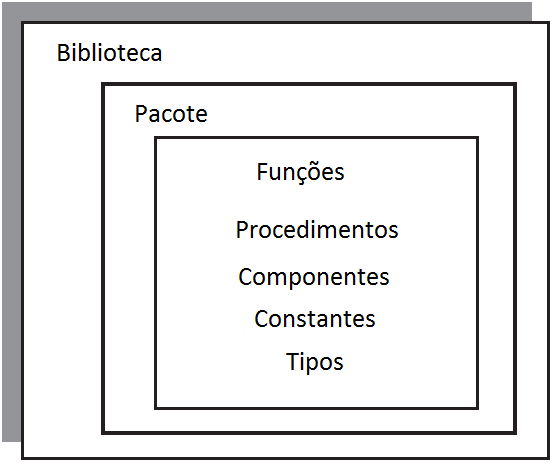
\includegraphics[scale=0.5]{library.png}
		\caption{Estrutura de uma Library \cite{Pedroni}}
		\label{library}
	\end{figure}
	
\subsection{Entidade}
Uma entidade de projeto pode representar uma simples porta l�gica como um sistema completo. A declara��o da entidade define a interface com o ambiente exterior, como, por exemplo, as entradas e sa�das. Os quatro modos de porta s�o:

	\begin{enumerate}
    	\item IN : Apenas entrada.
    	\item OUT: Apenas sa�da.
    	\item BUFFER: Sa�da que controla sinal interno.
		\item INOUT: Porta bidirecional    
	\end{enumerate}

	\begin{figure}[h] \centering
		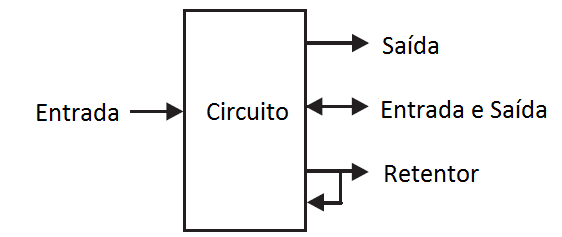
\includegraphics[scale=0.5]{entity.png}
		\caption{Tipos de Entrada e Sa�da \cite{Pedroni}}
		\label{entity}
	\end{figure}
	
\subsection{Arquitetura}
A arquitetura cont�m a parte l�gica da entidade utilizando suas entradas e sa�das. Ainda � poss�vel declarar sinais internos dentro da arquitetura, estes sinais s�o chamados classes. S�o elas:
	\begin{enumerate}
		\item CONSTANT - Define um objeto com valor est�tico.
		\item VARIABLE - S�o objetos que podem ter o seu valor alterado, e s�o usadas em regi�es de c�digo seq�encial.
		\item SIGNAL - S�o objetos que podem ter o seu valor alterado, e s�o usadas em regi�es de c�digo concorrente 				ou seq�encial. � bom lembrar que a porta de uma entidade realiza a declara��o de um sinal. 
	\end{enumerate}

	\begin{figure}[h] \centering
		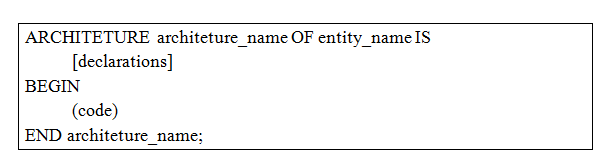
\includegraphics[scale=0.5]{architeture.png}
		\caption{Sintaxe de uma Architeture}
		\label{sintaxeArchiteture}
	\end{figure}

A arquitetura � composta de duas partes, uma para declara��es, onde sinais e constantes s�o declarados e outra onde fica o c�digo. Como no caso da entidade, o nome da arquitetura pode ser qualquer nome (exceto palavras reservadas), at� mesmo o nome da entidade.     	  %% Revisao Bibliogr�fica
% ----------------------------------------------------------------
% Desenvolvimento
% ----------------------------------------------------------------
\chapter{Desenvolvimento}

\section{Requisitos de Funcionamento}

% Descreve os sofwares necessarios para o projeto
\subsection{Software}
	
	\begin{itemize}
		\item Altera Quartus II Version 13.1 Build 162 09/02/2014 SJ Web Edition
		\item ModelSim Altera Starter Edition 13.1
		\item Sistema Operacional Windows 7/8/8.1
	\end{itemize}

% Descreve o hardware necessario para o projeto
\subsection{Hardware}

	\begin{itemize}
		\item Microcomputador de 1GHz ou superior
		\item 256 MB de Mem�ria RAM
		\item 4GB de espa�o dispon�vel em disco
	\end{itemize}
	
% Descreve as maquinas utilizadas no projeto
\subsection{Ferramentas Utilizadas no Projeto}

	\begin{itemize}
		\item Software Quartus II 13.1 Web Edition
		\item ModelSim Altera Starter Edition 13.1
		\item Notebook Dell Inspiron 14R: Intel Core i7, 8GB de Mem�ria RAM, 1TB de espa�o em disco.
		\item Notebook Samsung RF511-SD3BR: Intel Core i7, 8GB de Mem�ria RAM, 1TB de espa�o em disco.
	\end{itemize}
	
\section{Defini��o do Conjunto de Instru��es}

\subsection{Conjunto de Instru��es CISC}
	Em uma m�quina CISC, como o iAPX8086, h� centenas de instru��es de diversos tamanhos. Isso se justificava no passado pela velocidade lenta da mem�ria, uma vez que ap�s acess�-la para buscar uma instru��o a execu��o das demais instru��es normalmente n�o precisava de outro acesso.
	
	No entanto, as mem�rias de hoje s�o de alto desempenho, e dispensam a precau��o de evitar acess�-las. Diante disso, um programa CISC se torna complexo e demanda tempo para ser executado, uma vez que possui instru��es complexas que requerem v�rios ciclos de rel�gio e raramente s�o utilizadas.
	
	Um programa escrito para uma m�quina CISC, possui instru��es escritas de um modo menor, ou seja, est�o mais simples, por�m mais codificadas. Quando o processador recebe tais instru��es ele tem de decodific�-las em c�digo de m�quina para que seus circuitos possam execut�-las.
	
	Os processadores de arquitetura CISC cont�m uma micro-programa��o, ou seja, um conjunto de c�digos de instru��es que s�o gravados no processador. Desta forma, este recebe as instru��es dos programas e as executa utilizando as instru��es contidas em sua micro-programa��o. 
	
	A Figura \ref{FigFluxogramaCISC} a seguir ilustra o processo de quebra do c�digo que chega ao microprocessador, j� em baixo n�vel, em diversas instru��es mais pr�ximas do hardware, estas por sua vez est�o contidas no microc�digo do processador.
	
	\begin{figure}[ht] \centering
		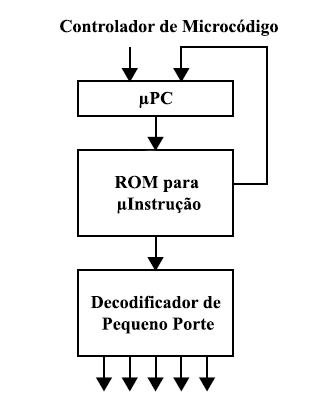
\includegraphics[scale=0.7]{fluxograma-maquina-cisc.jpg}
		\caption{Sequ�ncia para Execu��o de Instru��es CISC}
		\label{FigFluxogramaCISC}
	\end{figure}
	
\subsection{Conjunto de Instru��es RISC}
	Em uma m�quina RISC, como a desenvolvida neste trabalho, o conjunto de instru��es � reduzido. O hardware suporta um conjunto m�nimo de fun��es, sendo estas opera��es aritm�ticas e l�gicas, transfer�ncia de dados entre CPU, mem�ria e perif�ricos, al�m de opera��es de controle da m�quina.
	
	Uma das principais caracter�sticas das instru��es � que cada uma executa uma a��o muito simples. Assim, uma m�quina RISC tem suas instru��es compiladas diretamente para c�digo de m�quina, n�o sendo necess�ria uma posterior quebra em microc�digo (como ocorre em m�quinas CISC).
	
	A Figura \ref{FigFluxogramaRISC} a seguir ilustra o processo de compila��o dos programas de um microprocessador de arquitetura RISC.
	
	\begin{figure}[ht] \centering
		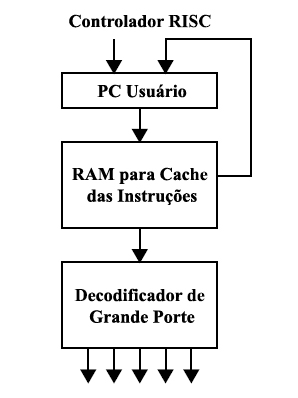
\includegraphics[scale=0.7]{fluxograma-maquina-risc.jpg}
		\caption{Sequ�ncia para Execu��o de Instru��es RISC}
		\label{FigFluxogramaRISC}
	\end{figure}
	
	A defini��o de um conjunto de instru��es para uma m�quina RISC segue as seguintes regras:	
	\begin{itemize}
		\item Analisar aplica��es para identificar opera��es-chave
		\item Projetar um processador que seja eficiente para executar essas opera��es.
		\item Projetar instru��es que realizam as opera��es-chave.
		\item Acrescentar mais instru��es necess�rias, cuidando para n�o afetar a velocidade da m�quina.
	\end{itemize}
	
\subsection{Instru��es Escolhidas}
	Para a implementa��o de um microprocessador o primeiro item que necessita ser pensado e desenvolvido com muita aten��o � o conjunto de instru��es, portanto dentre 255 instru��es do microprocessador 8086 foram escolhidas somente as instru��es que s�o de funcionamento b�sico de um programa de computador.

	Realizando um pararelo entre os dois tipos poss�veis de conjunto de instru��es, o microprocessador em desenvolvimento implementar� instru��es semelhantes ao conjunto do Microprocessador MIPS, que possui um conjunto de instru��es bem reduzido, somente com 50 instru��es e todos opcodes com o tamanho fixo de 6 bits, al�m que dentro dessas instru��es elas s�o subdividas em somente 3 tipos, que s�o: I,J e R. Sendo o tipo I, as opera��es de registro - imediato, as instru��es J, que s�o os jumps e as instru��es R, que s�o as instru��es registro-registro.

	``O design do conjunto de instru��es deve ter v�rios objetivos, sendo o mais �bvio e �til a performance do microprocessador.'' \cite{ArtigoVLSI}.

	Neste momento a preocupa��o � desenvolver um microprocessador que tenha um funcionamento b�sico e muito expl��cito, pois o foco deste trabalho n�o � desenvolver uma tecnologia nova, por�m compreender profundamente o desenvolvimento da arquitetura e dos componentes de um microprocessador e lembrando que, as m�quinas RISC s� se tornaram vi�veis devido aos avan�os de software no aparecimento de compiladores otimizados. \cite{ArtigoRisc}.

	Para adequar o 8086 a filosofia RISC, somente um modo de endere�amento � poss��vel, somente o modo imediato, pois torna o microprocessador uma m�quina Load/Store, nenhuma opera��o mem�ria-mem�ria se adequa a filosofia. Al�m do conjunto de instru��es caracter��stico, os microprocessadores RISC possuem normalmente uma grande quantidade de registradores, devidamente pela impossibilidade de realizar opera��es mem�ria-mem�ria, por�m o microprocessador a ser desenvolvido por seguir as caracter��sticas de um 8086, possuir� somente os mesmos registradores existentes no microprocessador 8086 CISC, em busca de facilitar o desenvolvimento, al�m disso, com o foco de que o mesmo c�digo gerado para um microprocessador 8086 CISC possa ser utilizado, claro sendo que sejam as mesmas instru��es, em sua vers�o RISC.

	Para o devido gerenciamento de mem�ria, o microprocessador a ser desenvolvido n�o ir� ter em seu conjunto os modos que fazem uso de segmenta��o, portanto a mem�ria ser� enxergada como uma mem�ria linear. Como se tivessemos somente um segmento sendo utilizado, tal defini��o ser� explicitada mais a diante. Semelhante ao funcionamento do micrprocessador 386 que possui al�m de um modo de mem�ria segmentada, um modo protegido o qual a mem�ria � vista linearmente.

	Portanto, ap�s todas as considera��es tomadas para o desenvolvimento do conjunto de instru��es, temos na Tabela \ref{tabelaInstrucoes} o conjunto de instru��es escolhido para o desenvolvimento deste microprocessador.

	\begin{table}[htbp]
		\centering
  		\caption{Instru��es Escolhidas e seus devidos Opcodes}
  		\begin{tabular}{|c|c|}
			\hline
			Instru��o & Opcode \\
			\hline
			\textbf{ADD  Reg16,Imed 16} & 10000001 11000 R/M I16L I16H \\
			\hline
			\textbf{OR     Reg16,Imed16} & 10000001 11001 R/M I16L I16H \\
			\hline
		    \textbf{ADC  Reg16,Imed16} & 10000001 11010 R/M I16L I16H \\
		    \hline
		    \textbf{SBB   Reg16,Imed16} & 10000001 11011 R/M I16L I16H \\
		    \hline
		    \textbf{AND  Reg16,Imed16} & 10000001 11100 R/M I16L I16H \\
		    \hline
		    \textbf{SUB   Reg16,Imed16} & 10000001 11101 R/M I16L I16H \\
		    \hline
		    \textbf{XOR   Reg16,Imed16} & 10000001 11110 R/M I16L I16H \\
		    \hline
		    \textbf{CMP  Reg16,Imed16} & 10000001 11111 R/M I16L I16H \\
		    \hline
		    \textbf{MOV Reg16,Imed16} & 00000000 10111 R/M I16L I16H \\
		    \hline
		\end{tabular}
		\label{tabelaInstrucoes}%
\end{table}%

	Para realizar uma verifica��o das instru��es escolhidas e determinar a sua finalidade, utilizou-se da libera��o que a Microsoft realizou nos �ltimos dias, que foi, abrir o c�digo fonte do sistema MS-DOS para o Museu da Hist�ria da Computa��o, o qual foi disponibilizado pela internet \cite{MSDOSLink}, neste arquivo que pode ser feito realizado o download livremente, existem duas vers�es do MS-DOS, como base utilizamos a vers�o 1.1 do MS-DOS, com os arquivos fontes escritos em Asembly. Baseado hist�ricamente, este sistema  era executado em um processador Intel�. Portanto, desenvolveu-se um c�digo na linguagem Python, que encontra-se em anexo, para realizar uma varredura em todos os arquivos .asm para checar a quantidade de instru��es semelhantes as que foram definidas como instru��es do microprocessador a ser implementado, com os resultados, se tem a Figura \ref{FigInstrucoes}.

	\begin{figure}[ht] \centering
		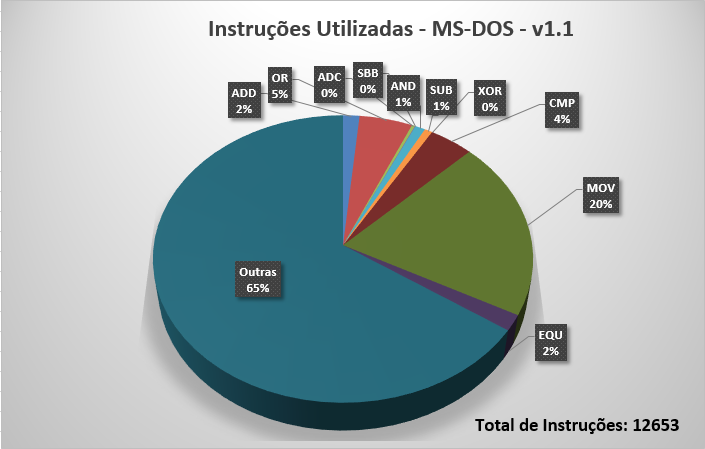
\includegraphics[scale=0.8]{instrucoesMSDOS.png}
		\caption{An�lise quantitativa das instru��es do c�digo do MS-DOS\cite{MSDOSLink}}
		\label{FigInstrucoes}
	\end{figure}

	Assim como em um projeto de pesquisa da IBM identificou que a maioria das instru��es eram usadas com pouca freq��ncia. Cerca de 20\% delas eram usadas 80\% das vezes. Os pr�prios desenvolvedores de sistemas operacionais habituaram-se a determinados subconjuntos de instru��es, tendendo a ignorar as demais, principalmente as mais complexas \cite{ArtigoRisc}, no gr�fico se v� claramente a alta utiliza��o de instru��es MOV, independente do seu tipo de endere�amento, o que a torna essencial ao processador aqui desenvolvido.

\subsection{Defini��o do Tamanho das Instru��es}
	Na arquitetura CISC h� instru��es de diversos tamanhos. Um exemplo � o iAPX8086, que cont�m instru��es que variam de 1 at� 6 bytes. Desta forma, cada uma destas instru��es requer uma quantidade diferente de ciclos de m�quina para serem executadas.
	
	Na arquitetura RISC todas as instru��es possuem o mesmo tamanho. E, segundo a regra de ouro, todas as instru��es devem ser executadas em apenas um ciclo de m�quina. O problema quanto � regra de ouro s�o as instru��es LOAD e STORE que requerem mais ciclos de rel�gio, uma vez que estas fazem acesso � mem�ria.
	
	Neste ponto, a regra de ouro tem de ser adaptada. A solu��o proposta � que a cada ciclo de rel�gio a execu��o de uma nova instru��o seja iniciada. E nessa caracter�stica � que entra o uso da t�cnica de pipelining.
	
	Para o microprocessador desenvolvido neste trabalho as instru��es possuem 4 bytes. Este tamanho de instru��o foi definido visando uma melhor administra��o da mem�ria dispon�vel e respeitando a regra de ouro, onde todas as instru��es tem o mesmo tamanho. Na Figura \ref{FigEstruturaInstrucao} a seguir tem-se a estrutura das instru��es aritm�ticas e l�gicas.
	
	\begin{figure}[ht] \centering
		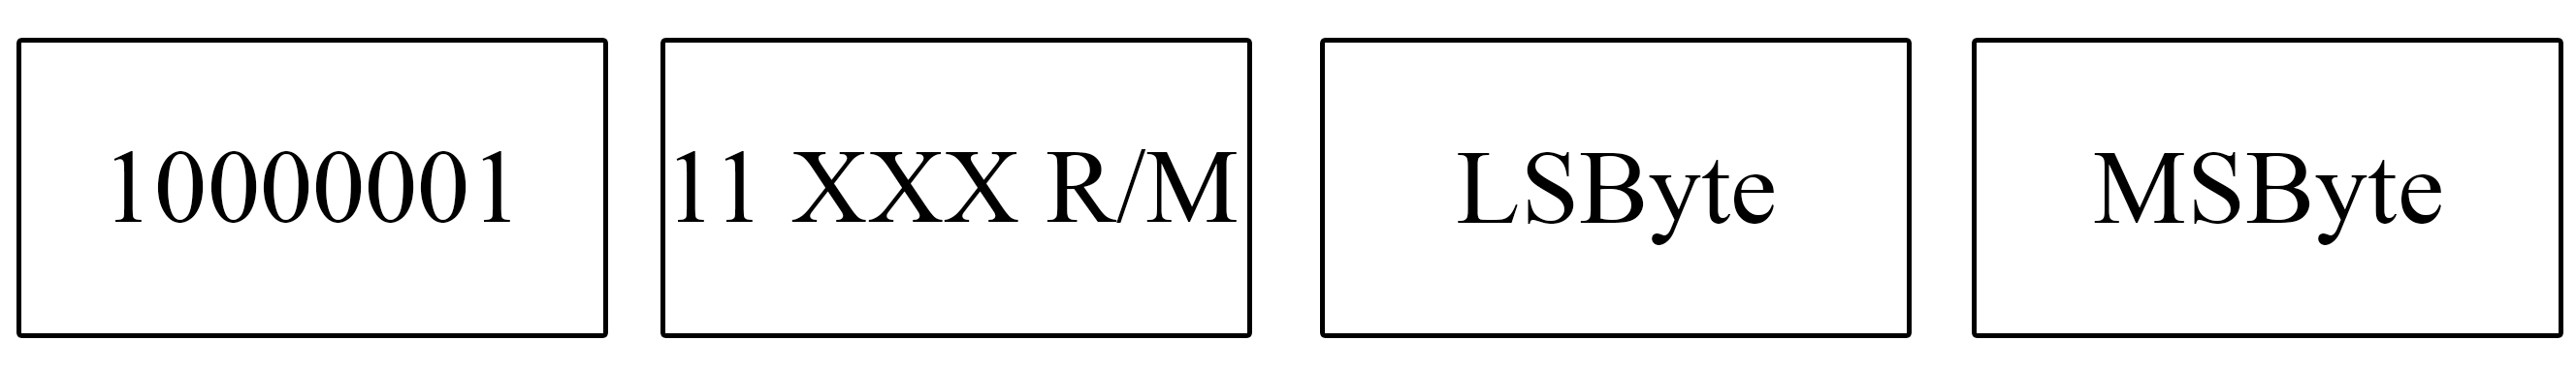
\includegraphics[scale=0.15]{estrutura_instrucao.jpg}
		\caption{Bytes das Instru��es Aritm�ticas e L�gicas}
		\label{FigEstruturaInstrucao}
	\end{figure}
	
	Na Figura \ref{FigEstruturaInstrucaoMOV} a seguir tem-se a estrutura da instru��o MOV.
	
	\begin{figure}[ht] \centering
		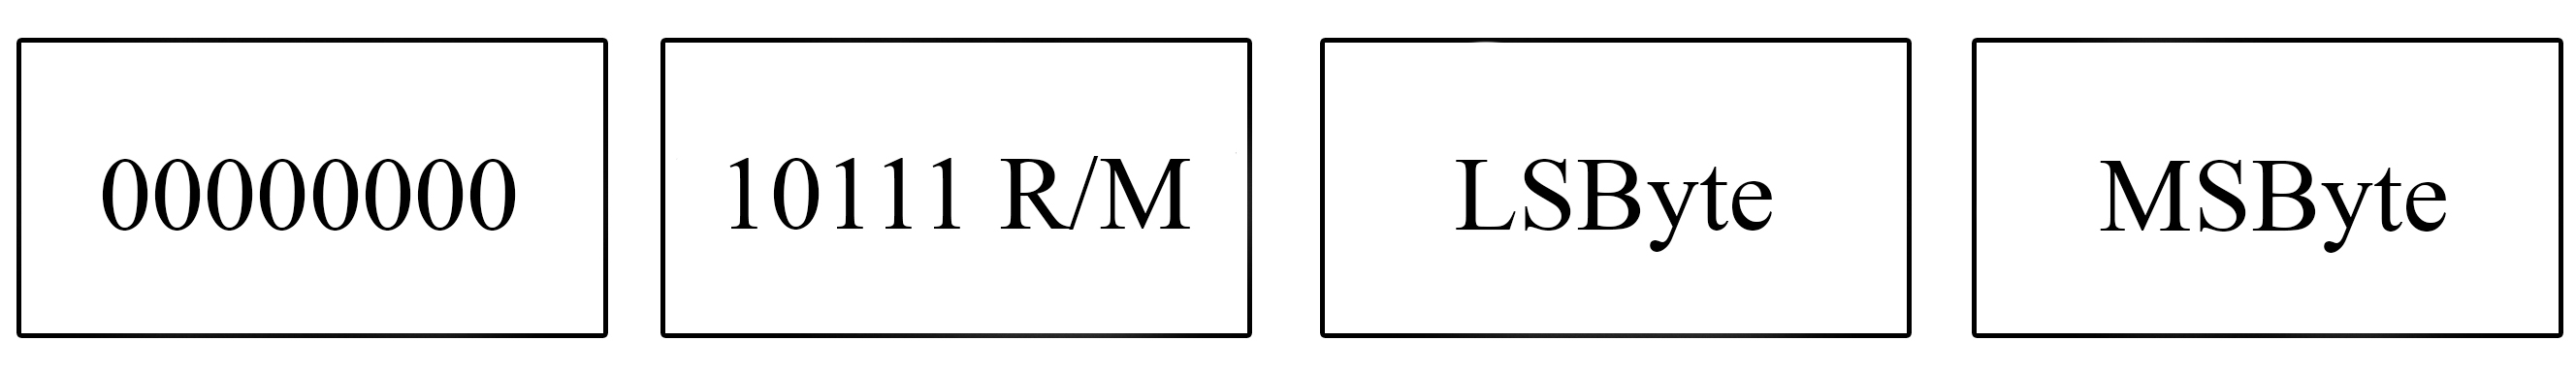
\includegraphics[scale=0.15]{estrutura_instrucao_mov.jpg}
		\caption{Bytes da Instru��o MOV}
		\label{FigEstruturaInstrucaoMOV}
	\end{figure}

\section{Implementa��o em VHDL}
	� seguir, ser� descrito todos os componentes em VHDL que foram desenvolvidos passo a passo, cada um com a sua devida valida��o com um testbench executado pelo Modelsim, todos os c�digos desenvolvidos es�o localizados em anexos.
	
\subsection{Registro de Prop�sito Geral}
	O registrador de pr�posito geral tem como objetivo encapsular os registradores AX, BX, CX, DX, SP, BP, SI e DI. Como definido anteriormente, todos os registro s�o de 16bits, portanto al�m de possuir entrada e sa�da de 16 bits, possui uma entrada de controle, para a sele��o correta do registrador desejado, que � determinado no opcode pelo item R/M, que segue por padr�o assim como no 8086 a tabela \ref{tabelaRegPropGeral}. Al�m de entradas para o \textit{clock} e \textit{reset} do sistema e uma entrada de controle de leitura/escrita, sendo leitura em n�vel baixo e escrita em n�vel alto, al�m da entrada de habilita��o do componente para o devido controle da m�quina de estados do microprocessador.
	
\begin{table}[htbp]
  \centering
  \caption{C�digos de controle do Registro de Prop�sito Geral}
    \begin{tabular}{|c|c|}
    	\hline
		\textbf{Registrador} & \textbf{C�digo R/M} \\
		\hline
	    \textbf{AX} & 000 \\
	    \hline
	    \textbf{BX} & 011 \\
	    \hline
	    \textbf{CX} & 001 \\
	    \hline
	    \textbf{DX} & 010 \\
    	\hline
	    \textbf{SP} & 100 \\
	    \hline
	    \textbf{BP} & 101 \\
	    \hline
    	\textbf{SI} & 110 \\
	    \hline
    	\textbf{DI} & 111 \\
	    \hline
	\end{tabular}%
	\label{tabelaRegPropGeral}%
\end{table}%
	
Temos na Figura \ref{figRegPropositoGeralTB} o resultado produzido pela execu��o do \textit{testbench}, que tamb�m se encontra em anexos.
	
	\begin{figure}[ht] \centering
		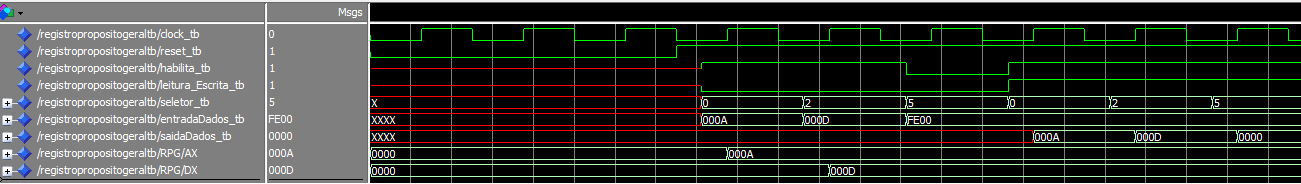
\includegraphics[scale=0.5]{printsImplementacaoVHDL/regPropositoGeralTB.png}
		\caption{Resultado do \textit{testbench} aplicado ao componente de Registro de Prop�sito Geral}
		\label{figRegPropositoGeralTB}
	\end{figure}
	
\subsection{Registro de Segmento}
	Com funcionamento semelhante do Registro de Prop�sito Geral, possui o objetivo de encaplusar os registradores que possuem o funcionamento de manipula��o de mem�ria que s�o, CS, ES, DS, SS, al�m do contador de �ndice IP. Diferentemente, do Registro de Pop�sito Geral, o registro de Segmento, possui uma linha de entrada denominada incrementa\_IP, tal linha foi implementada a fim de facilitar o comando de incremento de IP para se caminhar continuamente na mem�ria, sendo que o registro possui acesso direto ao registrador IP, em vez de se desenvolver uma estrutura pr�pria para este c�lculo. Tal registro tamb�m possui seu devido barramento de controle de 3 bits, que est� descrito na Tabela \ref{tabelaRegSeg}, por�m como descrito anteriormente este barramento ser� fixado em "001" para que somente seja utilizado o segmento de c�digo para o funcionamento deste microprocessador.
	
\begin{table}[htbp]
  \centering
  \caption{C�digos de controle do Registro de Segmento}
    \begin{tabular}{|c|c|}
    	\hline
		\textbf{Registrador} & \textbf{C�digo R/M} \\
		\hline
	    \textbf{ES} & 000 \\
	    \hline
	    \textbf{CS} & 001 \\
	    \hline
	    \textbf{SS} & 010 \\
	    \hline
	    \textbf{DS} & 010 \\
	    \hline
	    \textbf{IP} & 100 \\
	    \hline
    	\textbf{Todos em Alta Imped�ncia} & outros \\
    	\hline
    \end{tabular}%
  \label{tabelaRegSeg}%
\end{table}%

	Temos na Figura \ref{figRegSegmentoTB} o resultado produzido pela execu��o do \textit{testbench}, que tamb�m se encontra em anexos.
	
	\begin{figure}[ht] \centering
		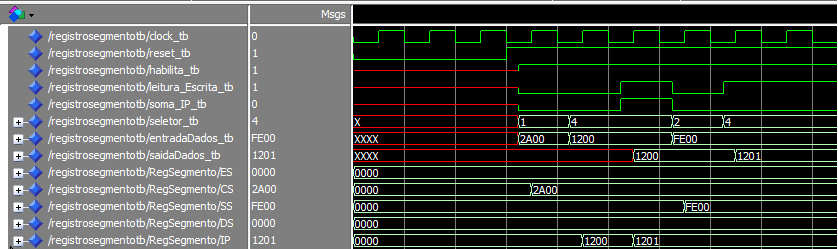
\includegraphics[scale=0.7]{printsImplementacaoVHDL/regSegmentoTB.png}
		\caption{Resultado do \textit{testbench} aplicado ao componente de Registro de Segmento}
		\label{figRegSegmentoTB}
	\end{figure}

\subsection{Calculadora de Endere�o}

	Foi desenvolvido uma calculadora de endere�o para realizar o c�lculo do endere�o relativo para o endere�o f�sico, por exemplo, temos o seguinte endere�o l�gico CS:IP, sendo CS com 1200h e IP com 3450h, ent�o, a calculado tem o papel de converter este endere�o l�gico, realizando a seguinte opera��o: 12000h + 3405h = 15405h, um endere�o f�sico de 16 bits que � colocado no barramento de endere�o do microprocessador, a fim de apontar um endere�o na mem�ria. Assim foi desenvolvido um componente simples, com duas entradas de 16 bits e uma sa�da de 20 bits, temos na Figura \ref{figCalcEndTB} a execu��o do exemplo dado logo a cima.	 

	\begin{figure}[ht] \centering
		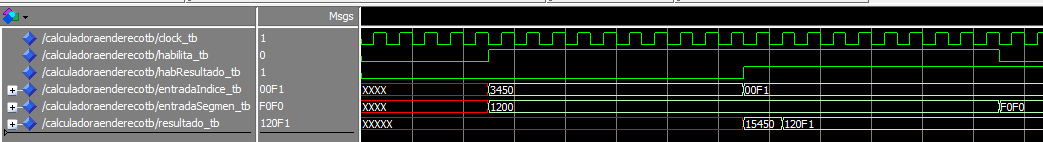
\includegraphics[scale=0.5]{printsImplementacaoVHDL/calcEndTB.png}
		\caption{Resultado do \textit{testbench} aplicado a Calculadora de Endere�o}
		\label{figCalcEndTB}
	\end{figure}

\subsection{Demultiplexador}
	O Demultiplexador seleciona um dos diversos dados de entrada e o transfere para a sa�da. Foi implementado para possuir duas sa�das de 16 bits, devido requisitos b�sicos do sistema.

	\begin{figure}[ht] \centering
		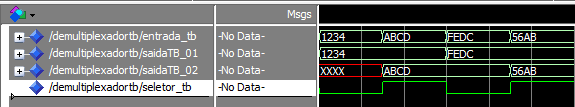
\includegraphics[scale=1]{printsImplementacaoVHDL/demuxTB.png}
		\caption{Resultado do \textit{testbench} aplicado ao Demultiplexador}
		\label{figDemuxTB}
	\end{figure}

\subsection{Multiplexador}
	O Multiplexador seleciona um dos diversos dados de entrada e o transfere para a sa�da. Assim como o Demultiplexador, foi implementado com duas entradas de 16 bits.
	
	\begin{figure}[ht] \centering
		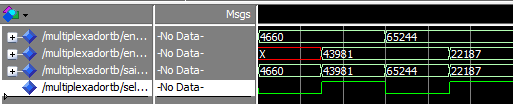
\includegraphics[scale=1]{printsImplementacaoVHDL/muxTB.png}
		\caption{Resultado do \textit{testbench} aplicado ao Multiplexador}
		\label{figMuxTB}
	\end{figure}

\subsection{Registro de Flags} 
	O Registro de Flags tem como objetivo guardar o resultado dos flags que s�o calculado pela Unidade L�gica Aritm�tica. Funciona como um flip-flop para cada sinal de entrada, por�m como sa�da possui um �nico vetor de 16 bits, para que tenha uma exibi��o semelhante � maneira de se manipular flags no microprocessador 8086, podemos verificar seu funcionamento na Figura \ref{figRegFlagTB}.

	\begin{figure}[ht] \centering
		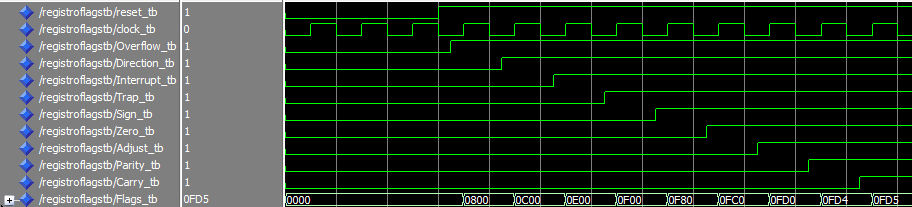
\includegraphics[scale=0.7]{printsImplementacaoVHDL/registroFlagsTB.png}
		\caption{Resultado do \textit{testbench} aplicado ao Registro de Flags}
		\label{figRegFlagTB}
	\end{figure}

\subsection{Unidade de Controle de Endere�os}
	A Unidade de Controle de Endere�os possui como objetivo controlar alguns componentes a maneira de realizar a perfeita sincroniza��o entre eles, e que exista um fluxo consistente de dados entre as estruturas para que o c�lculo que seja realizado, e que seja correto.
	Portanto a Unidade de Controle de Endere�os � a implementa��o de uma m�quina de estados \ref{figUCEestados}, que � iniciada em reset, e estimulado por pulsos de clock e por um sinal de habilita��o advindo da Unidade de Controle, respons�vel pela realiza��o da sincronia total do microprocessador.
	
	\subsubsection{Diagrama de Estados}	
	\begin{figure}[ht] \centering
		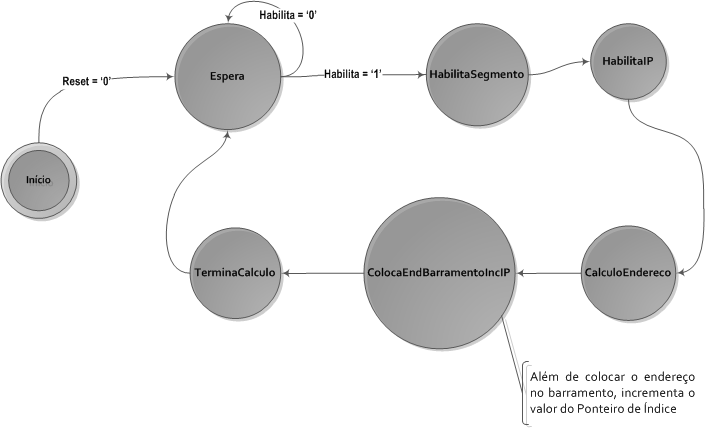
\includegraphics[scale=0.8]{DiagramaEstadosEnd.png}
		\caption{Diagrama de Estados da Unidade de Controle de Endere�os}
		\label{figUCEestados}
	\end{figure}
	
	O sinal de habilita existe para que exista uma esp�cie de dom�nio da Unidade de Controle sobre a Unidade de Controle de Endere�os, pois o papel da controladora de endere�os � fornecer � mem�ria o endere�o correto para que a unidade de controle sempre acesse no barramento de dados, um dado v�lido para que a m�quina n�o trave e sempre continue processando c�clicamente, temos na Figura \ref{figUCETB} o resultado do \textit{testbench} realizado com a unidade.
	
\subsection{Mem�ria ROM}
	A mem�ria ROM � utilizada para armazenar os opcodes das instru��es. Os valores armazenados na estrutura representam o que seria o resultado da compila��o de um software. Desta forma, esta � utilizada para simula��o da funcionalidade do microprocessador diante de um c�digo assembly resultante do processo de compila��o.
	
	Na Figura \ref{saidaMemoriaROM} abaixo tem-se a simula��o da funcionalidade desta estrutura:
	
	\begin{figure}[ht] \centering
		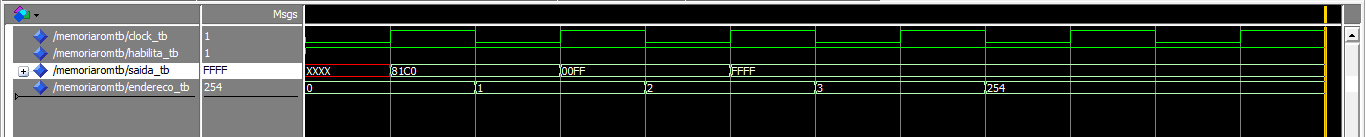
\includegraphics[scale=0.3]{printsImplementacaoVHDL/print_memoria_rom.jpg}
		\caption{Sa�da Mem�ria ROM}
		\label{saidaMemoriaROM}
	\end{figure}
	
\subsection{Unidade Aritm�tica e L�gica - ULA}
	� a estrutura respons�vel por executar todas as opera��es aritm�ticas e l�gicas do microprocessador. � composta por algumas estruturas auxiliares, j� descritas neste documento, que implementam funcionalidades necess�rias na execu��o bit a bit de cada instru��o. Os dados chegam na ULA atrav�s do multiplexador ou direto da unidade de controle, a respectiva opera��o � executada e ent�o o resultado � colocado no registrador correspondente definido pela unidade de controle.

	
	\begin{figure}[ht] \centering
		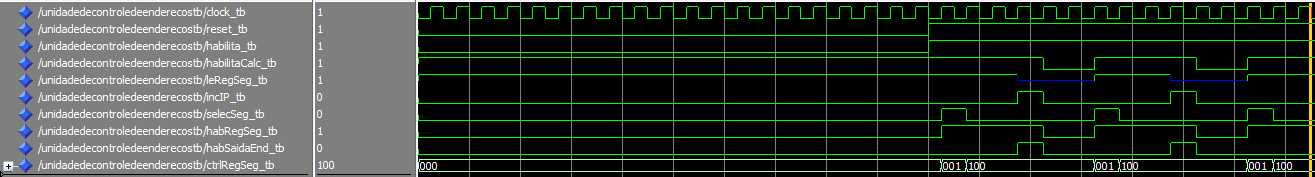
\includegraphics[scale=0.5]{printsImplementacaoVHDL/unidadeControleEndTB.png}
		\caption{Resultado do \textit{testbench} aplicado a Unidade de Controle de Endere�os}
		\label{figUCETB}
	\end{figure}

\subsubsection{Detector do Flag Auxiliar}
	O Detector do Flag Auxiliar � uma estrutura criada para ser utilizada na Unidade Aritm�tica e L�gica. Esta estrutura detecta a ocorr�ncia de um "vai um" do bit 3 para o bit 4 ou quando h� "vem um" do bit 4 para o bit 3, durante a execu��o de alguma instru��o aritm�tica.
	A valida��o da funcionalidade da estrutura atrav�s de um \textit{testbench} � apresentada na Figura \ref{saidaAuxiliarFlag} a seguir:
	
	\begin{figure}[ht] \centering
		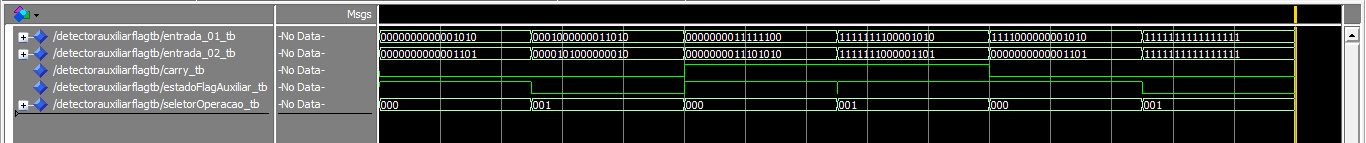
\includegraphics[scale=0.3]{printsImplementacaoVHDL/print_detector_auxiliar_flag.jpg}
		\caption{Sa�da Estrutura Detector Auxiliar Flag}
		\label{saidaAuxiliarFlag}
	\end{figure}
	
\subsubsection{Detector do Flag de Paridade}
	O Detector do Flag de Paridade � uma estrutura que detecta a paridade do resultado obtido em uma instru��o aritm�tica ou l�gica. � utilizado na Unidade Aritm�tica e L�gica. Caso haja um n�mero par de bits 1 no resultado da opera��o, o flag de paridade recebe valor 1, caso contr�rio, recebe valor 0.
	Na Figura \ref{saidaFlagParidade} a seguir, tem-se a valida��o da funcionalidade da estrutura:
	
	\begin{figure}[ht] \centering
		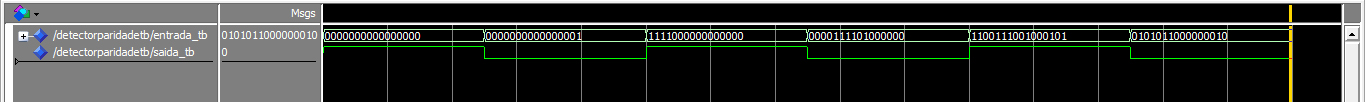
\includegraphics[scale=0.3]{printsImplementacaoVHDL/print_detector_paridade.jpg}
		\caption{Sa�da Estrutura Detector Flag de Paridade}
		\label{saidaFlagParidade}
	\end{figure}
	
\subsubsection{Detector do Zero Flag}
	Esta estrutura verifica o resultado obtido em uma opera��o aritm�tica ou l�gica. Caso o valor final seja 0, o zero flag recebe valor 1, caso contr�rio, recebe valor 0.
	Na Figura \ref{saidaZeroParidade} a seguir se tem a valida��o da funcionalidade da estrutura:
	
	\begin{figure}[ht] \centering
		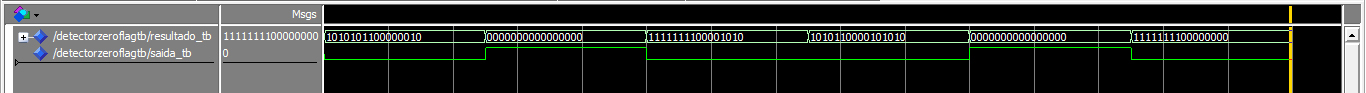
\includegraphics[scale=0.3]{printsImplementacaoVHDL/print_detector_zero_flag.jpg}
		\caption{Sa�da Estrutura Detector Zero Flag}
		\label{saidaZeroParidade}
	\end{figure}

	
\subsection{Unidade de Controle}
	A Unidade de Controle � uma das principais estruturas do microprocessador. Ela � respons�vel por 3 fun��es b�sicas: busca (fetch), decodifica��o e execu��o. Al�m disso, gera todos os sinais que controlam as unidades \textit{escravas} � ela. A \textit{Unidade de Controle de Endere�os} � uma m�quina de estados escrava � unidade de controle, portanto h� um sinal de habilita��o que conecta essas duas unidades que � enviado pela Unidade de Controle, tornando-a uma m�quina de estados \textit{master}. Podemos verificar o diagrama de estados implementado na Unidade de Controle, na Figura \ref{diagramaUC}.
	
	\begin{figure}[ht] \centering
		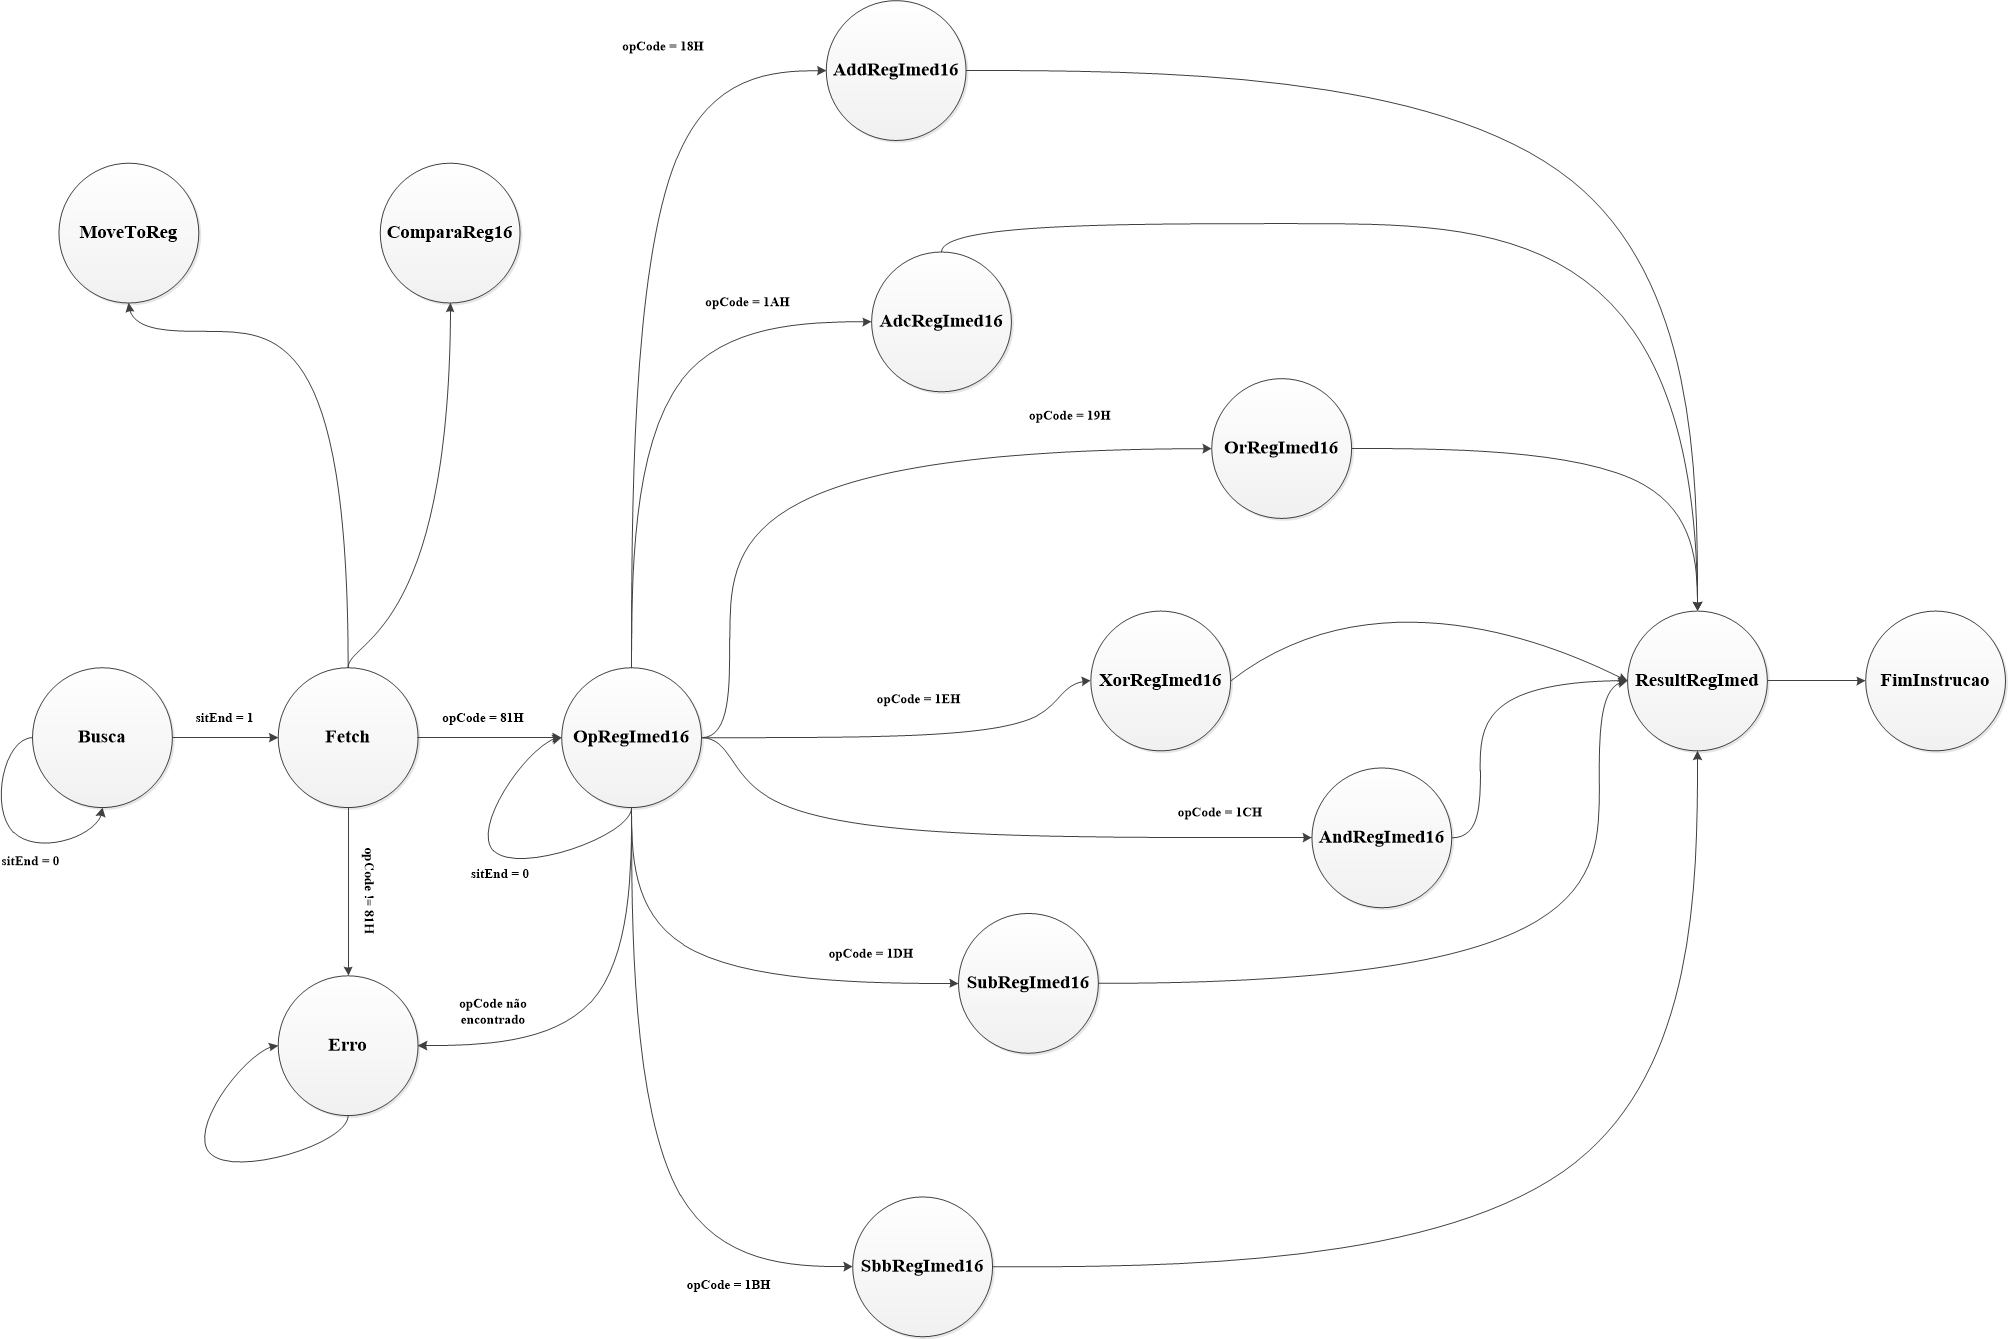
\includegraphics[scale=0.25]{diagrama_estados_unidade_controle.jpg}
		\caption{Diagrama de Estados da Unidade de Controle}
		\label{diagramaUC}
	\end{figure}    
%\chapter{Resultados}
O processador implementado foi testado da seguinte maneira, foi criado um arquivo \textit{testbench} e atrav�s dos resultados fornecidos pelo software ModelSim - Altera, selecionando somente os sinais internos de interesse da instru��o, que ser� colocada diretamente no barramento de dados, em sua forma hexadecimal. 
Nas pr�ximas se��es, ser�o detalhadas todas as instru��es implementadas, uma a uma com o seu devido resultado do \textit{testbench}.

Temos na Figura \ref{FigTestes}, a vis�o RTL da estrutura de simula��o que � a conex�o de uma mem�ria ROM que possui o c�digo a ser executado e o microprocessador.
	\begin{figure} \centering
		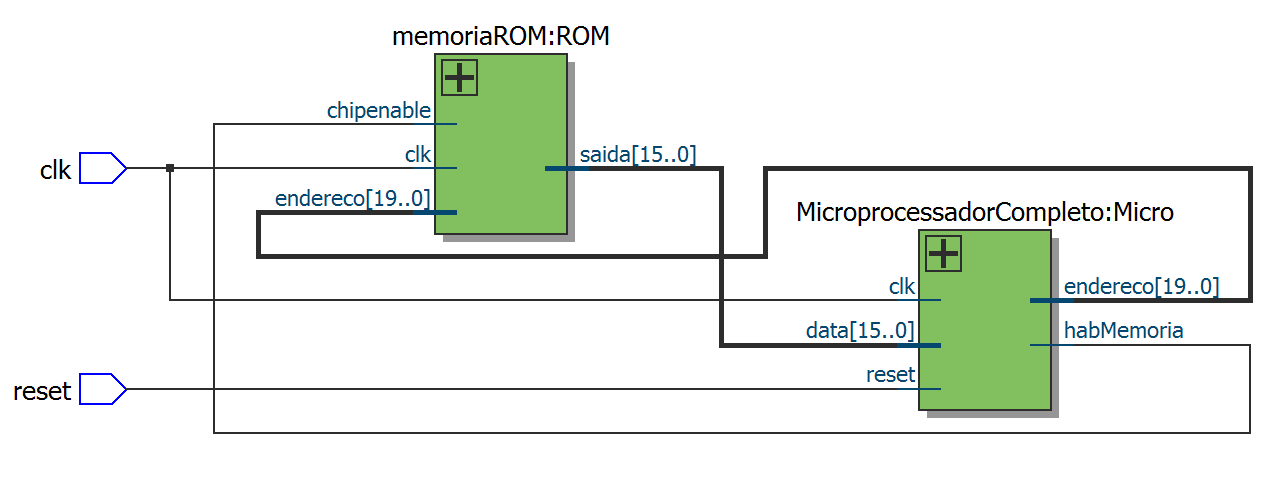
\includegraphics[scale=0.35]{imagensResultados/estruturaTesteMicroROM.png}
		\caption{Vis�o RTL da estrutura de testes}
		\label{FigTestes}
	\end{figure}

Temos na Figura \ref{FigMicroFinal}, a vis�o RTL da estrutura do microprocessador completo, com todas as estruturas e liga��es necess�rias para o perfeito funcionamento.

\begin{figure} \centering
		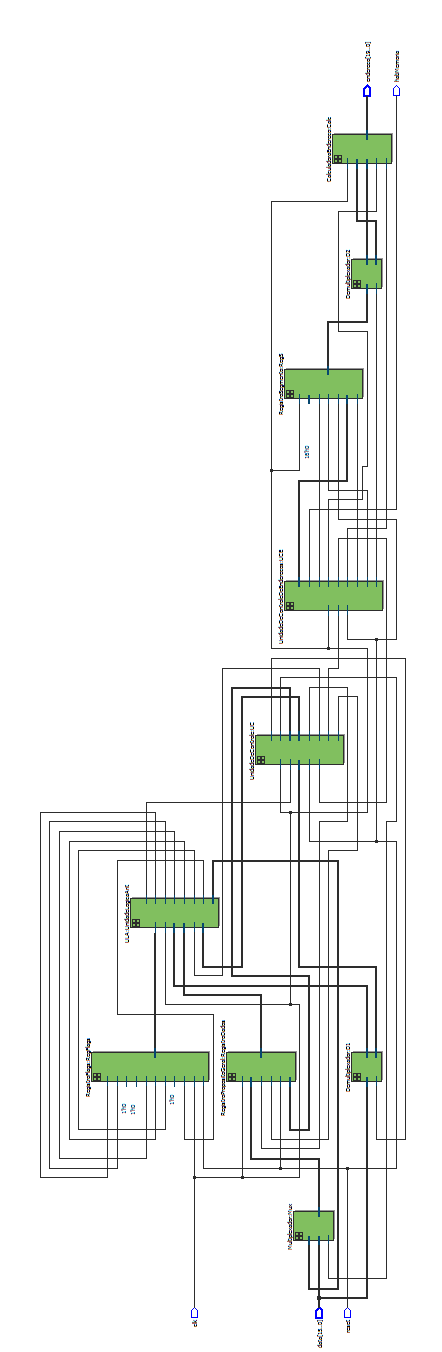
\includegraphics[scale=0.65]{imagensResultados/microRISCFinalRTL.png}
		\caption{Vis�o RTL do microprocessador com todas estruturas corretas e funcionais}
		\label{FigMicroFinal}
	\end{figure}
\begin{figure} \centering
		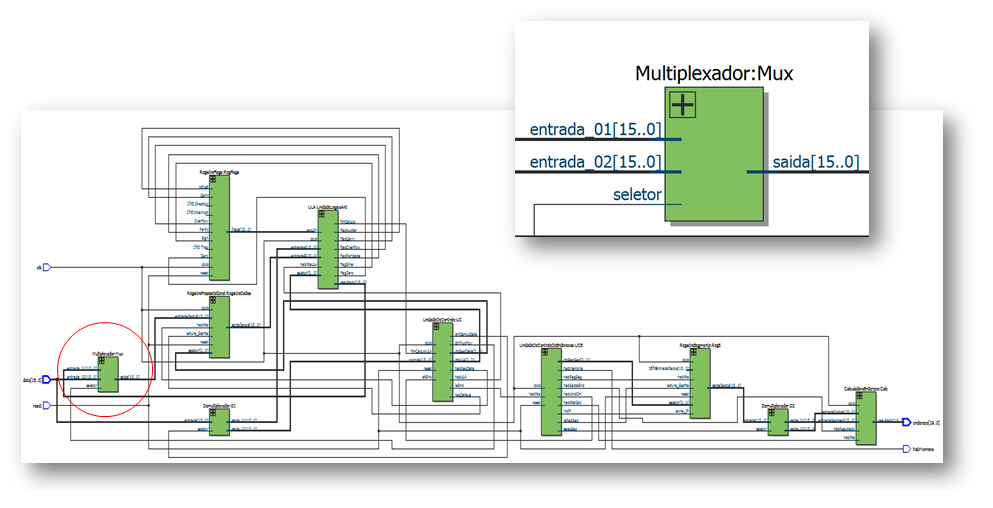
\includegraphics[scale=0.65]{imagensResultados/focoMux.png}
		\caption{Vis�o RTL do microprocessador com foco no Multiplexador}
		\label{FigMicroFinal}
	\end{figure}
\begin{figure} \centering
		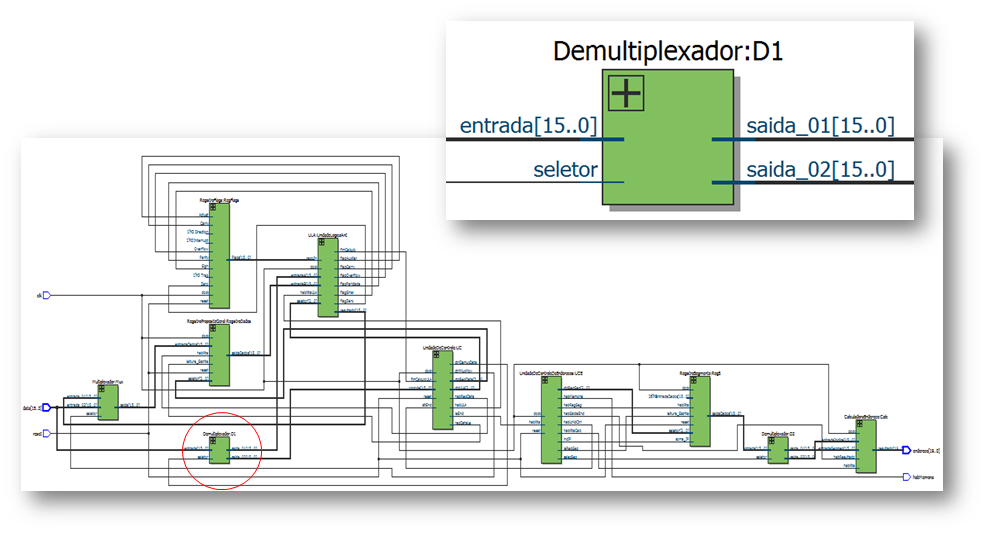
\includegraphics[scale=0.65]{imagensResultados/focoDemux.png}
		\caption{Vis�o RTL do microprocessador com foco no Demultiplexador}
		\label{FigMicroFinal}
	\end{figure}
\begin{figure} \centering
		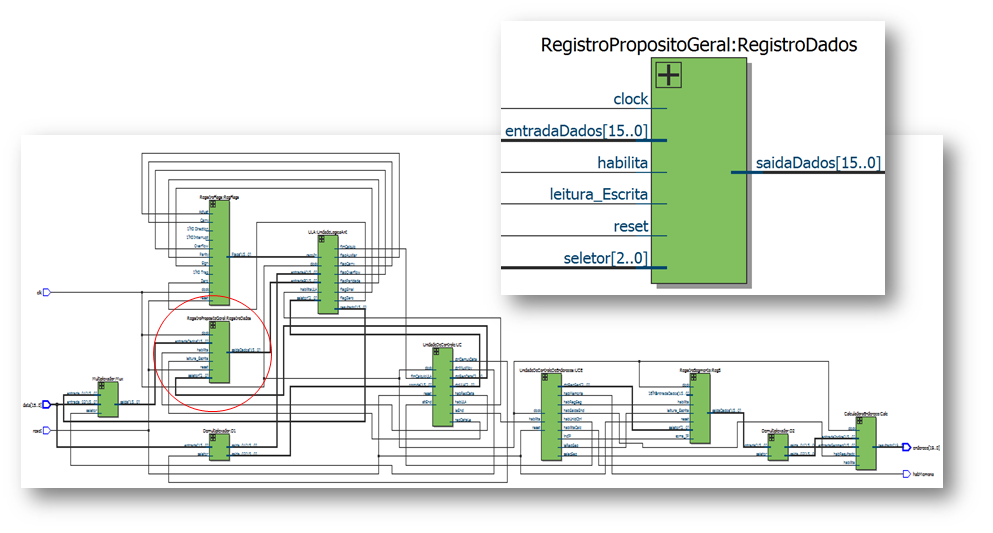
\includegraphics[scale=0.65]{imagensResultados/focoRegDados.png}
		\caption{Vis�o RTL do microprocessador com foco no Registro de Dados}
		\label{FigMicroFinal}
	\end{figure}
\begin{figure} \centering
		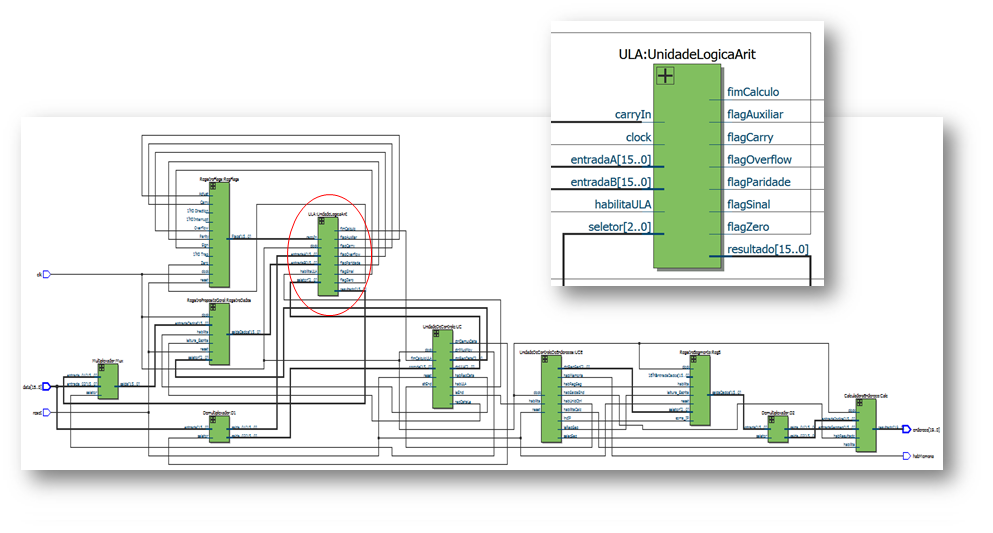
\includegraphics[scale=0.65]{imagensResultados/focoULA.png}
		\caption{Vis�o RTL do microprocessador com foco na Unidade L�gica Aritm�tica}
		\label{FigMicroFinal}
	\end{figure}
\begin{figure} \centering
		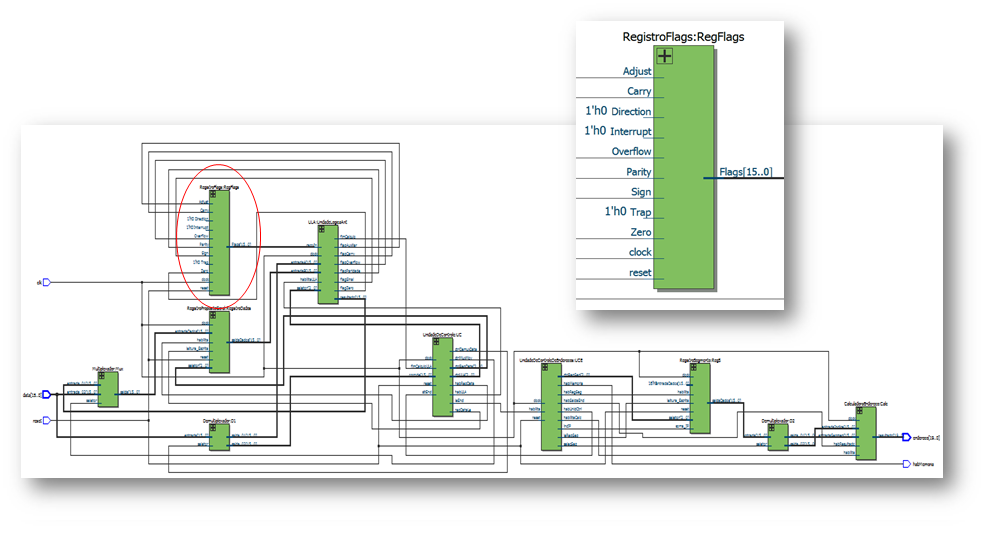
\includegraphics[scale=0.65]{imagensResultados/focoFlags.png}
		\caption{Vis�o RTL do microprocessador com foco no Registro de Flags}
		\label{FigMicroFinal}
	\end{figure}
\begin{figure} \centering
		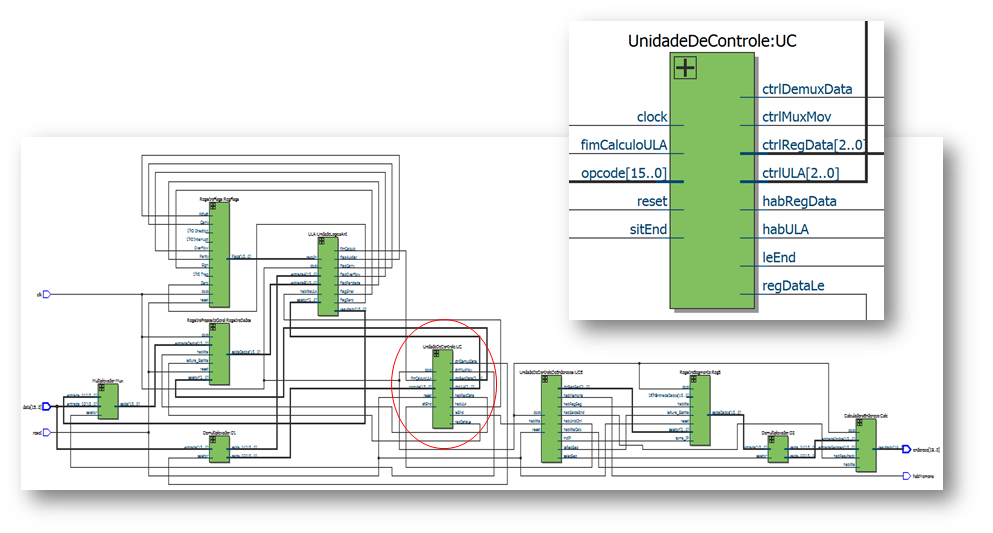
\includegraphics[scale=0.65]{imagensResultados/focoUC.png}
		\caption{Vis�o RTL do microprocessador com foco na Unidade de Controle}
		\label{FigMicroFinal}
	\end{figure}
\begin{figure} \centering
		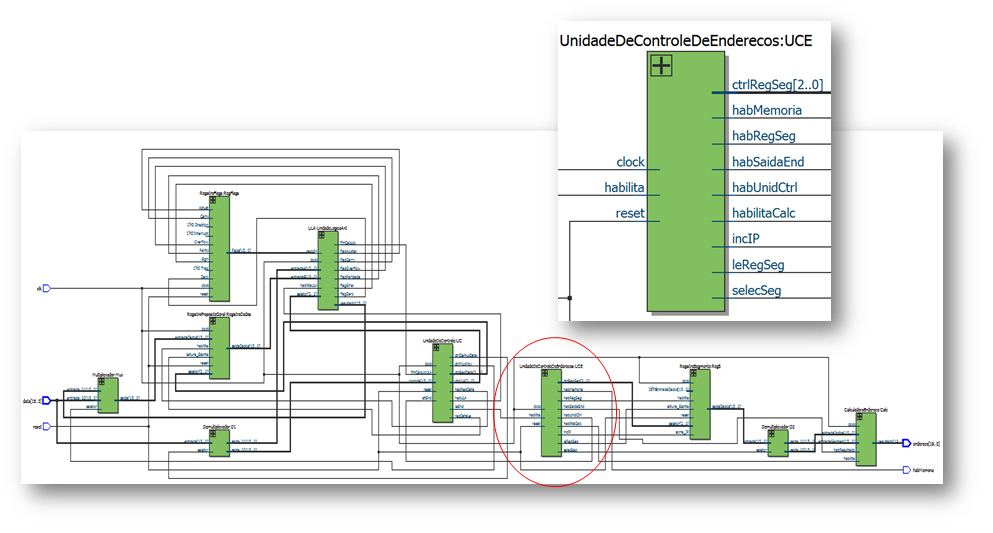
\includegraphics[scale=0.65]{imagensResultados/focoUCE.png}
		\caption{Vis�o RTL do microprocessador com foco na Unidade de Controle de Endere�o}
		\label{FigMicroFinal}
	\end{figure}
\begin{figure} \centering
		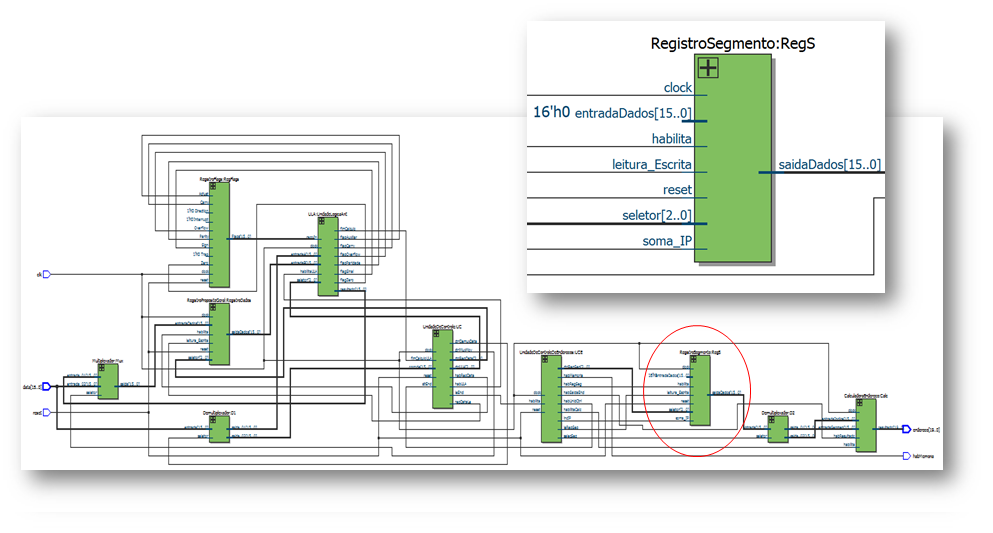
\includegraphics[scale=0.65]{imagensResultados/focoRegSeg.png}
		\caption{Vis�o RTL do microprocessador com foco no Registro de Segmento}
		\label{FigMicroFinal}
	\end{figure}
\begin{figure} \centering
		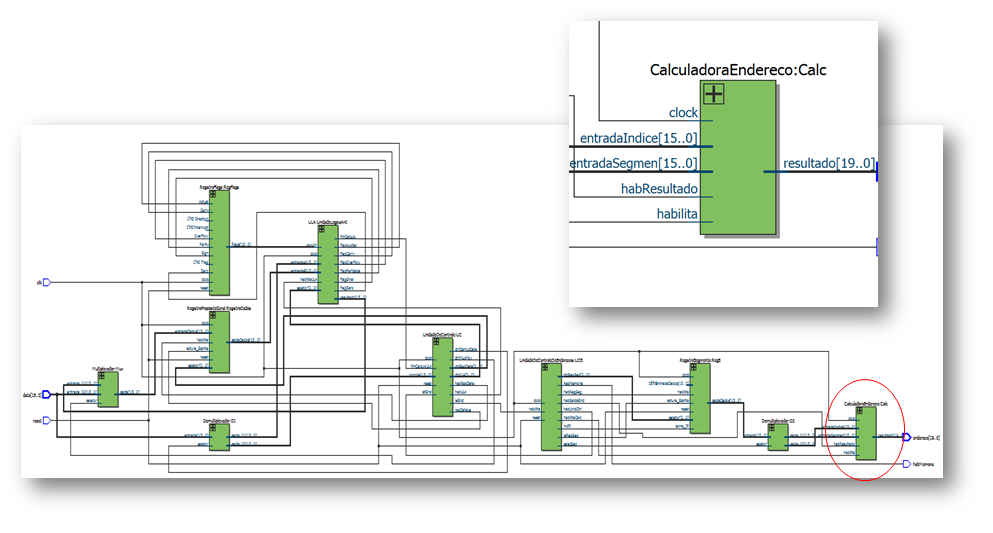
\includegraphics[scale=0.65]{imagensResultados/focoCalc.png}
		\caption{Vis�o RTL do microprocessador com foco na Calculadora de Endere�o}
		\label{FigMicroFinal}
	\end{figure}
	
\section{ADD Reg16,Imed16}
Esta instru��o adiciona ao valor do registro um valor imediato de 16 bits, a instru��o de teste em hexadecimal � definida como \textbf{81C0 00FF}, sendo 81C0h o opcode da instru��o e 00FFh o valor imediato a ser somado no registro AX, por utilizar R/M igual a 000 como visto anteriormente. Na Figura \ref{FigResultAdd} � poss�vel ver o resultado da execu��o do \textit{testbench}, com os sinais que mais interessam no funcionamento tanto da mem�ria quanto do microprocessador para esta opera��o, as linhas de rel�gio e reset s�o respons�veis pelo funcionamento passo a passo do microprocessador, tanto que enquanto a linha de reset n�o fica em n�vel alto, o microprocessador n�o responde. Tem-se os sinais dos estados da Unidade de Controle e da Unidade de Controle de Endere�o, �teis para verificar se a linha de racioc�nio, presente nos grafos descritos anteriormente, est� correta e respeitando a ordem de mestre e escravo imposta. O endere�o e a sa�da da mem�ria ROM, exteriorizadas de maneira a verificar se o microprocessador est� colocando no barramento de endere�o o valor correto e se a mem�ria coloca no barramento de dados o valor correto do \textit{opcode}. Al�m disso, o enumerado descrito na Unidade L�gica e Aritm�tica para verificar qual opera��o � realizada dentro deste componente, � poss�vel notar que esta linha se mantem em  \textbf{op\_add}, e por fim o registrador AX, o qual est� sendo manipulado, para se verificar a altera��o em seu valor. Pode-se perceber que a instru��o est� funcionando corretamente, pois o valor do registrador AX � alterado para \textbf{00FFh} ap�s a execu��o da instru��o e todos os estados s�o percorridos, como realmente deveria ser em ambas unidades de controle.

\begin{landscape}
	\begin{figure}
		\includegraphics[scale=0.5]{imagensResultados/OperacaoAdd.png}
		\caption{Resultado Teste Opera��o ADD}
		\label{FigResultAdd}
	\end{figure}
\end{landscape}

\section{OR Reg16,Imed16}
Esta instru��o realiza a opera��o ``OU''  bit a bit do valor do registro com um valor imediato de 16 bits, a instru��o de teste em hexadecimal � definida como \textbf{81C8 1234}, sendo 81C8h o opcode da instru��o e 1234h o valor imediato a ser realizado a opera��o ``OU'' no registro AX, por utilizar R/M igual a 000 como visto anteriormente. Na Figura \ref{FigResultOr} tem-se o resultado da execu��o do \textit{testbench}, com os sinais que mais interessam no funcionamento tanto da mem�ria quanto do microprocessador para esta opera��o, as linhas de rel�gio e reset s�o respons�veis pelo funcionamento e passo a passo do microprocessador, tanto que enquanto a linha de reset n�o fica em n�vel alto, o microprocessador n�o responde. Os sinais dos estados da Unidade de Controle e da Unidade de Controle de Endere�o, �teis para verificar se a linha de racioc�nio, presente nos grafos descritos anteriormente, est� correta e respeitando a ordem de mestre e escravo imposta. Temos o endere�o e a sa�da da mem�ria ROM, exteriorizadas de maneira a verificar se o microprocessador est� colocando no barramento de endere�o o valor correto e se a mem�ria coloca no barramento de dados o valor correto do \textit{opcode}. Al�m disso, tem-se o enumerado descrito na Unidade L�gica e Aritm�tica para verificar qual opera��o � realizada dentro deste componente, pode-se ver que esta linha � alterada para \textbf{op\_a\_or\_b}, e por fim tem-se o registrador AX, o qual est� sendo manipulado, para se verificar a altera��o em seu valor. Pode-se verificar que a instru��o est� funcionando corretamente, pois o valor do registrador AX � alterado para \textbf{1234h} ap�s a execu��o da instru��o e todos os estados s�o percorridos, como realmente deveriam ser em ambas unidades de controle.

\begin{landscape}
	\begin{figure}
		\includegraphics[scale=0.5]{imagensResultados/OperacaoOr.png}
		\caption{Resultado Teste Opera��o OR}
		\label{FigResultOr}
	\end{figure}
\end{landscape}

\section{ADC Reg16,Imed16}
Esta instru��o adiciona, com carry, ao valor do registro um valor imediato de 16 bits, a instru��o de teste em hexadecimal � definida como \textbf{81D0 1234}, sendo 81D0h o opcode da instru��o e 1234h o valor imediato a ser somado com carry no registro AX, por utilizar R/M igual a 000 como visto anteriormente. Na Figura \ref{FigResultAdc} pode-se ver o resultado da execu��o do \textit{testbench}, com os sinais que interessam no funcionamento tanto da mem�ria quanto do microprocessador para esta opera��o. As linhas de rel�gio e reset s�o respons�veis pelo funcionamento passo a passo do microprocessador, tanto que enquanto a linha de reset n�o fica em n�vel alto, o microprocessador n�o responde. Os sinais dos estados da Unidade de Controle e da Unidade de Controle de Endere�o, �teis para verificar se a linha de racioc�nio, presente nos grafos descritos anteriormente, est� correta e respeitando a ordem de mestre e escravo imposta. Tem-se o endere�o e a sa�da da mem�ria ROM, exteriorizadas de maneira a verificar se o microprocessador est� colocando no barramento de endere�o o valor correto e se a mem�ria coloca no barramento de dados o valor correto do \textit{opcode}. Tem-se tamb�m a utiliza��o do sinal de \textit{carryIn} que � colocado em n�vel alto, em busca de verificar a diferen�a entre esta opera��o e a opera��o de soma sem o \textit{carry}. Al�m disso, o enumerado descrito na Unidade L�gica e Aritm�tica verifica qual opera��o � realizada dentro deste componente. Assim, � poss�vel notar que esta linha � alterada para \textbf{op\_addCarry}, e por fim tem-se o registrador AX, o qual est� sendo manipulado, para verificar a altera��o em seu valor. � poss�vel perceber que a instru��o est� funcionando corretamente, pois o valor do registrador AX � alterado para \textbf{1235h} ap�s a execu��o da instru��o e todos os estados s�o percorridos, como realmente deveria ser em ambas unidades de controle.

\begin{landscape}
	\begin{figure}
		\includegraphics[scale=0.5]{imagensResultados/OperacaoAdc.png}
		\caption{Resultado Teste Opera��o ADC}
		\label{FigResultAdc}
	\end{figure}
\end{landscape}

\section{SBB Reg16,Imed16}
Esta instru��o subtrai, com borrow, ao valor do registro um valor imediato de 16 bits, a instru��o de teste em hexadecimal � definida como \textbf{81D8 1234}, sendo 81D8h o opcode da instru��o e 1234h o valor imediato a ser subtra�do com borrow no registro AX, por utilizar R/M igual a 000 como visto anteriormente. Na Figura \ref{FigResultSbb} pode-se ver o resultado da execu��o do \textit{testbench}, com os sinais que mais interessam no funcionamento tanto da mem�ria quanto do microprocessador para esta opera��o, as linhas de rel�gio e reset s�o respons�veis pelo funcionamento passo a passo do microprocessador, tanto que enquanto a linha de reset n�o fica em n�vel alto, o microprocessador n�o responde. Tem-se os sinais dos estados da Unidade de Controle e da Unidade de Controle de Endere�o, �teis para verificar se a linha de racioc�nio, presente nos grafos descritos anteriormente, est� correta e respeitando a ordem de mestre e escravo imposta. Tem-se o endere�o e a sa�da da mem�ria ROM, exteriorizadas de maneira a verificar se o microprocessador est� colocando no barramento de endere�o o valor correto e se a mem�ria coloca no barramento de dados o valor correto do \textit{opcode}. Tem-se tamb�m a utiliza��o do sinal de \textit{carryIn}, que neste caso � utilizado como borrow, � colocado em n�vel alto, em busca de verificar a diferen�a entre esta opera��o e a opera��o de subtra��o sem o \textit{borrow}. Al�m disso, o enumerado descrito na Unidade L�gica e Aritm�tica para se verificar qual opera��o � realizada dentro deste componente, sendo poss�vel notar que esta linha se mantem em  \textbf{op\_subCarry}, e por fim tem-se o registrador AX, o qual est� sendo manipulado, para se verificar a altera��o em seu valor. Pode-se verificar que a instru��o est� funcionando corretamente, pois o valor do registrador AX � alterado para \textbf{EDCBh} ap�s a execu��o da instru��o e todos os estados s�o percorridos, como realmente deveria ser em ambas unidades de controle.

\begin{landscape}
	\begin{figure}
		\includegraphics[scale=0.5]{imagensResultados/OperacaoSbb.png}
		\caption{Resultado Teste Opera��o SBB}
		\label{FigResultSbb}
	\end{figure}
\end{landscape}

\section{AND Reg16,Imed16}
Esta instru��o realiza a opera��o ``AND''  bit a bit do valor do registro com um valor imediato de 16 bits, a instru��o de teste em hexadecimal � definida como \textbf{81E0 1234}, sendo 81E0h o opcode da instru��o e 1234h o valor imediato a ser realizado na opera��o ``AND'' com o registro AX, por utilizar R/M igual a 000 como visto anteriormente. Na Figura \ref{FigResultAnd} pode-se ver o resultado da execu��o do \textit{testbench}, com os sinais que mais interessam no funcionamento tanto da mem�ria quanto do microprocessador para esta opera��o, as linhas de rel�gio e reset s�o respons�veis pelo funcionamento  passo a passo do microprocessador, tanto que enquanto a linha de reset n�o fica em n�vel alto, o microprocessador n�o responde. Nos sinais dos estados da Unidade de Controle e da Unidade de Controle de Endere�o, �teis para verificar se a linha de racioc�nio, presente nos grafos descritos anteriormente, est� correta e respeitando a ordem de mestre e escravo imposta. Tem-se o endere�o e a sa�da da mem�ria ROM, exteriorizadas de maneira a verificar se o microprocessador est� colocando no barramento de endere�o o valor correto e se a mem�ria coloca no barramento de dados o valor correto do \textit{opcode}. Al�m disso, o enumerado descrito na Unidade L�gica e Aritm�tica verifica qual opera��o � realizada dentro deste componente, podendo notar que esta linha se mantem em  \textbf{op\_a\_and\_b}, e por fim tem-se o registrador AX, o qual est� sendo manipulado, para verificar a altera��o em seu valor. Pode-se verificar que a instru��o est� funcionando corretamente, pois o valor do registrador AX � alterado para \textbf{0000h} ap�s a execu��o da instru��o e todos os estados s�o percorridos, como realmente deveria ser em ambas unidades de controle.

\begin{landscape}
	\begin{figure}
		\includegraphics[scale=0.5]{imagensResultados/OperacaoAnd.png}
		\caption{Resultado Teste Opera��o AND}
		\label{FigResultAnd}
	\end{figure}
\end{landscape}

\section{SUB Reg16,Imed16}
Esta instru��o subtrai ao valor do registro um valor imediato de 16 bits, a instru��o de teste em hexadecimal � definida como \textbf{81E8 1234}, sendo 81E8h o opcode da instru��o e 1234h o valor imediato a ser subtra�do no registro AX, por utilizar R/M igual a 000 como visto anteriormente. Na Figura \ref{FigResultSub} pode-se ver o resultado da execu��o do \textit{testbench}, com os sinais que mais  interessam no funcionamento tanto da mem�ria quanto do microprocessador para esta opera��o, as linhas de rel�gio e reset s�o respons�veis pelo funcionamento passo a passo do microprocessador, tanto que enquanto a linha de reset n�o fica em n�vel alto, o microprocessador n�o responde. Tem-se os sinais dos estados da Unidade de Controle e da Unidade de Controle de Endere�o, �teis para verificar se a linha de racioc�nio, presente nos grafos descritos anteriormente, est� correta e respeitando a ordem de mestre e escravo imposta. Tem-se o endere�o e a sa�da da mem�ria ROM, exteriorizadas de maneira a verificar se o microprocessador est� colocando no barramento de endere�o o valor correto e se a mem�ria coloca no barramento de dados o valor correto do \textit{opcode}. Al�m disso, o enumerado descrito na Unidade L�gica e Aritm�tica para verificar qual opera��o � realizada dentro deste componente, sendo poss�vel notar que esta linha se mantem em  \textbf{op\_sub}, e por fim tem-se o registrador AX, o qual est� sendo manipulado, para se verificar a altera��o em seu valor. Pode-se verificar que a instru��o est� funcionando corretamente, pois o valor do registrador AX � alterado para \textbf{EDCCh} ap�s a execu��o da instru��o e todos os estados s�o percorridos, como realmente deveria ser em ambas unidades de controle.

\begin{landscape}
	\begin{figure}
		\includegraphics[scale=0.5]{imagensResultados/OperacaoSub.png}
		\caption{Resultado Teste Opera��o SUB}
		\label{FigResultSub}
	\end{figure}
\end{landscape}

\section{XOR Reg16,Imed16}
Esta instru��o realiza a opera��o ``XOR''  bit a bit do valor do registro com um valor imediato de 16 bits, a instru��o de teste em hexadecimal � definida como \textbf{81E8 1234}, sendo 81E8h o opcode da instru��o e 1234h o valor imediato a ser realizado a opera��o ``XOR''  com o registro AX, por utilizar R/M igual a 000 como visto anteriormente. Na Figura \ref{FigResultXor}, tem-se o resultado da simula��o com os sinais que mais interessam no funcionamento tanto da mem�ria quanto do microprocessador. Para esta opera��o, as linhas de rel�gio e reset s�o respons�veis pelo funcionamento passo a passo do microprocessador, tanto que enquanto a linha de reset n�o fica em n�vel alto, o microprocessador n�o responde. Os sinais dos estados da Unidade de Controle e da Unidade de Controle de Endere�o, �teis para verificar se a linha de racioc�nio, presente nos grafos descritos anteriormente, est� correta e respeitando a ordem de mestre e escravo imposta. Tem-se o endere�o e a sa�da da mem�ria ROM, exteriorizadas de maneira a verificar se o microprocessador est� colocando no barramento de endere�o o valor correto e se a mem�ria coloca no barramento de dados o valor correto do \textit{opcode}. Al�m disso, o enumerado descrito na Unidade L�gica e Aritm�tica para verificar qual opera��o � realizada dentro deste componente, sendo poss�vel notar que esta linha se mantem em  \textbf{op\_a\_xor\_b}, e por fim tem-se o registrador AX, o qual est� sendo manipulado, para se verificar a altera��o em seu valor. Pode-se verificar que a instru��o est� funcionando corretamente, pois o valor do registrador AX � alterado para \textbf{1234h} ap�s a execu��o da instru��o e todos os estados s�o percorridos, como realmente deveria ser em ambas unidades de controle.

\begin{landscape}
	\begin{figure}
		\includegraphics[scale=0.5]{imagensResultados/OperacaoXor.png}
		\caption{Resultado Teste Opera��o XOR}
		\label{FigResultXor}
	\end{figure}
\end{landscape}

\section{CMP Reg16,Imed16}
Esta instru��o realiza a compara��o ao valor do registro um valor imediato de 16 bits, a instru��o de teste em hexadecimal � definida como \textbf{81F8 1234}, sendo 81F8h o opcode da instru��o e 1234h o valor imediato a ser comparado com o registro AX, por utilizar R/M igual a 000 como visto anteriormente. Na Figura \ref{FigResultComp}, tem-se o resultado da simula��o com os sinais que mais interessam no funcionamento tanto da mem�ria quanto do microprocessador. Para esta opera��o, as linhas de rel�gio e reset s�o respons�veis pelo funcionamento passo a passo do microprocessador, tanto que enquanto a linha de reset n�o fica em n�vel alto, o microprocessador n�o responde. Os sinais dos estados da Unidade de Controle e da Unidade de Controle de Endere�o, �teis para verificar se a linha de racioc�nio, presente nos grafos descritos anteriormente, est� correta e respeitando a ordem de mestre e escravo imposta. Tem-se o endere�o e a sa�da da mem�ria ROM, exteriorizadas de maneira a verificar se o microprocessador est� colocando no barramento de endere�o o valor correto e se a mem�ria coloca no barramento de dados o valor correto do \textit{opcode}. Al�m disso, o enumerado descrito na Unidade L�gica e Aritm�tica para verificar qual opera��o � realizada dentro deste componente, sendo poss�vel notar que esta linha se mantem em  \textbf{op\_a\_comp\_b}. � poss�vel perceber que todos os flags v�o para n�vel l�gico ``1'' ou ``0'', de acordo ao resultado da opera��o. Pode-se verificar que a instru��o est� funcionando corretamente, pois todos os estados s�o percorridos, como realmente deveria ser em ambas unidades de controle e, al�m disso, os flags utilizados para tomada de decis�o est�o com os valores corretos.

\begin{landscape}
	\begin{figure}
		\includegraphics[scale=0.5]{imagensResultados/OperacaoCmp.png}
		\caption{Resultado Teste Opera��o CMP}
		\label{FigResultComp}
	\end{figure}
\end{landscape}

\section{MOV Reg16,Imed16}
Esta instru��o move um valor imediato de 16 bits para um determinador registrador, a instru��o de teste em hexadecimal � definida como \textbf{00B8 1234}, sendo 00B8h o opcode da instru��o e 1234h o valor imediato a ser movido para o registro AX, por utilizar R/M igual a 000 como visto anteriormente. Na Figura \ref{FigResultMov}, tem-se o resultado da simula��o com os sinais que mais interessam no funcionamento tanto da mem�ria quanto do microprocessador. Para esta opera��o, as linhas de rel�gio e reset s�o respons�veis pelo funcionamento passo a passo do microprocessador, tanto que enquanto a linha de reset n�o fica em n�vel alto, o microprocessador n�o responde. Os sinais dos estados da Unidade de Controle e da Unidade de Controle de Endere�o, �teis para verificar se a linha de racioc�nio, presente nos grafos descritos anteriormente, est� correta e respeitando a ordem de mestre e escravo imposta. Tem-se o endere�o e a sa�da da mem�ria ROM, exteriorizadas de maneira a verificar se o microprocessador est� colocando no barramento de endere�o o valor correto e se a mem�ria coloca no barramento de dados o valor correto do \textit{opcode}. Al�m disso, pode-se perceber que os estados correspondentes ao funcionamento da instru��o MOV s�o percorridos corretamente desde o \textit{Fetch} at� \textit{Fim\_Move\_To\_Reg}, sendo que neste ponto o valor 1234h foi carregado no registrador AX.

\begin{landscape}
	\begin{figure}
		\includegraphics[scale=0.5]{imagensResultados/OperacaoMov.png}
		\caption{Resultado Teste Opera��o MOV}
		\label{FigResultMov}
	\end{figure}
\end{landscape}

% ----------------------------------------------------------------
% Consideracoes Finais e Trabalhos Futuros
% ----------------------------------------------------------------

\chapter{Considera��es Finais}

	Este trabalho tinha como objetivo desenvolver um processador RISC a partir de um originalmente feito na arquitetura CISC. Sendo poss�vel assim, analisar quest�es de desempenho no que diz respeito a execu��o dos programas e acessos � mem�ria. Poucas instru��es foram implementadas, uma vez que a arquitetura RISC possui um conjunto de instru��es curto e, al�m disso, este � um projeto com fins did�ticos sendo poss�vel, caso necess�rio, a implementa��o de mais instru��es posteriormente.
	
	O processador desenvolvido foi testado via simula��o e funcionou como esperado. As instru��es implementadas desempenharam corretamente sua fun��o e, portanto, pode-se dizer que o projeto foi conclu�do com �xito.
	
	Al�m disso o projeto foi desenvolvido de forma modular, o que facilita a manuten��o do c�digo e posteriores melhorias. Al�m disso, possui uma arquitetura de f�cil entendimento o que incentiva a continua��o do projeto em trabalhos futuros.
	
	O desenvolvimento deste trabalho foi muito importante na consolida��o dos conhecimentos de hardware e software. O estudo de como as diferentes arquiteturas das m�quinas s�o implementadas foi necess�rio, para definir o comportamento do processador aqui desenvolvido. Todo o processo de descri��o do comportamento destes blocos em VHDL requer um profundo conhecimento de t�cnicas de depura��o e desempenho na �rea de software e hardware.

\chapter{Trabalhos Futuros}

	A m�quina desenvolvida neste trabalho n�o teve todo o seu potencial implementado. � poss�vel desenvolver mais instru��es, respeitando a arquitetura RISC, de modo a dar maior flexibilidade na hora de escrever programas para o processador executar.

	H� tamb�m a possibilidade de aumentar o tamanho dos registros, desde que a filosofia da arquitetura utilizada seja respeitada, e melhorar o tamanho dos barramentos de comunica��o, tornando o processador mais poderoso.
	
	Al�m de que o microprocessador desenvolvido em n�vel de descri��o de hardware pode ser utilizado como base para futuros trabalhos nas �reas de \textit{pipeline}, \textit{placement}, \textit{routing}, entre outras pesquisas que necessitam da utiliza��o de um microprocessador simulado de f�cil compreens�o. Toda a documenta��o deste microprocessador est� em um reposit�rio aberto no Github, segue o endere�o: https://github.com/macaufreitas/micro-risc , assim liberamos o acesso a todos que desejam acessar qualquer documento diretamente do nosso desenvolvimento do projeto, al�m de liberar para a comunidade uma arquitetura de microprocessador \textit{open source}.
%\include{TrabalhosFuturos}
% ----------------------------------------------------------------
% Anexos
% ----------------------------------------------------------------
\chapter{Anexo}

\lstinputlisting[language = VHDL,title={Descri��o do hardware do Multiplexador}]{codigos/Multiplexador.vhd}

\lstinputlisting[language = VHDL,title={Descri��o do hardware do Demultiplexador}]{codigos/Demultiplexador.vhd}

\lstinputlisting[language = VHDL,title={Descri��o do hardware do Registro de Segmento}]{codigos/RegistroSegmento.vhd}

\lstinputlisting[language = VHDL,title={Descri��o do hardware do Registro de Prop�sito Geral}]{codigos/RegistroPropositoGeral.vhd}

\lstinputlisting[language = VHDL,title={Descri��o do hardware do Registro de Flags}]{codigos/RegistroFlags.vhd}

\lstinputlisting[language = VHDL,title={Descri��o do hardware da Calculadora de Endere�os}]{codigos/CalculadoraEndereco.vhd}

\lstinputlisting[language = VHDL,title={Descri��o do hardware do Detector de Flag Auxiliar}]{codigos/DetectorAuxiliarFlag.vhd}

\lstinputlisting[language = VHDL,title={Descri��o do hardware do Detector de Flag de Paridade}]{codigos/DetectorParidade.vhd}

\lstinputlisting[language = VHDL,title={Descri��o do hardware do Detector de Zero Flag}]{codigos/DetectorZeroFlag.vhd}

\lstinputlisting[language = VHDL,title={Descri��o do hardware da Unidade L�gica Aritm�tica - ULA}]{codigos/ULA.vhd}

\lstinputlisting[language = VHDL,title={Pacote auxiliar que descreve os estados da Unidade de Controle de Endere�os}]{codigos/uce_aux.vhd}

\lstinputlisting[language = VHDL,title={Descri��o do hardware da Unidade de Controle de Endere�os}]{codigos/UnidadeDeControleDeEnderecos.vhd}

\lstinputlisting[language = VHDL,title={Pacote auxiliar que descreve os estados da Unidade de Controle}]{codigos/uc_aux.vhd}

\lstinputlisting[language = VHDL,title={Descri��o do hardware da Unidade de Controle Principal}]{codigos/UnidadeDeControle.vhd}

\lstinputlisting[language = Python,title={C�digo em Python utilizado para a an�lise quantitativa do c�digo fonte do MS-DOS}]{codigos/ler_instrucoes_dos_v4.py}					  %% Anexos
% ----------------------------------------------------------------
\bibliographystyle{abntex2-alf}

\bibliography{biblio}             %% REFER�NCIAS (deve-se possuir o arquivo do tipo bibtex)
% ----------------------------------------------------------------
\end{document}
% ----------------------------------------------------------------